\chapter{Simulation Workflow}
\label{chap:workflow}

%%%%%%%%%%%%%%%%%%%%%%%%%%%%%%%%%%%%%%%%%%%%%%%%%%%%%%%%%%%%%%%%%%%%%%%%%%%%%%%%
\section{A Simulation Triad}
\label{chap4:triad}

This thesis investigates Monte Carlo as a means to generate multi-group cross sections for fine mesh transport codes. This work required the development of a ``simulation triad'' encompassing three primary codes as illustrated in Fig.~\ref{fig:chap4-simulation-triad}. First, the OpenMC Monte Carlo code~\cite{romano2013openmc} was utilized to generate multi-group cross sections. Second, the \ac{MGXS} were used by the OpenMOC \ac{MOC} code~\cite{boyd2014openmoc} for deterministic multi-group transport calculations. Finally, the OpenCG library~\cite{boyd2015opencg} enabled the processing and transfer of tally data on combinatorial geometry (CG) meshes between OpenMC and OpenMOC. In addition, a significant amount of infrastructural code was developed to process the results produced by OpenMC and OpenMOC. The results in this thesis may be most easily reproduced with the versions of OpenMC, OpenMOC and OpenCG itemized in Tab.~\ref{table:chap4-git-shas}.

\begin{table}[hb!]
  \centering
  \caption[OpenMC, OpenMOC and OpenCG Git SHA-1 hashes]{The Git SHA-1 commit hashes for each code used in this thesis.}
  \small
  \label{table:chap4-git-shas} 
  \vspace{6pt}
  \begin{tabular}{l c c}
  \toprule
  \rowcolor{lightgray}
  {\bf Code} &
  {\bf Date [MM-DD-YYYY]} &
  {\bf Git Commit SHA-1} \\
  \midrule
  OpenMC & 05-30-2016 & 698c223482a7d5f5df4dc83eeed65d99a2e52fbf \\
  OpenMOC\footnotemark & 05-29-2016 & b09e66be269703ca0a08d7a6afced1bc5984112a \\
  OpenCG & 05-14-2016 & 2c5e8f92f501d076f4ed06b70b09684a411b06b9 \\
  \bottomrule
\end{tabular}
\end{table}

\footnotetext{OpenMOC was compiled with double precision floating point arithmetic.}

\begin{figure}[h]
  \centering
  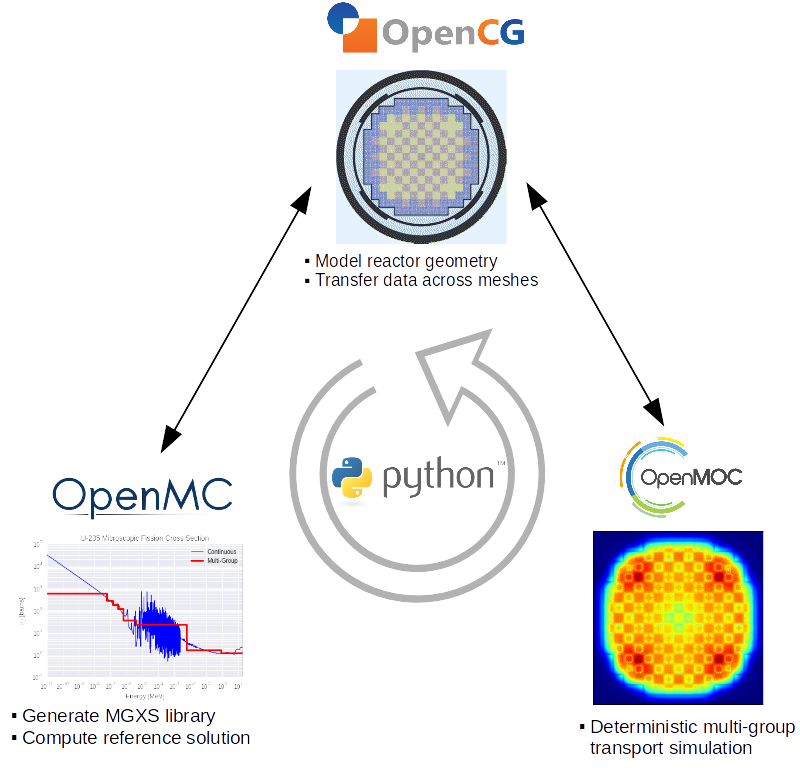
\includegraphics[width=0.8\linewidth]{figures/workflow/triad/simulation-triad}
\caption[A simulation triad of OpenMC, OpenMOC and OpenCG]{A simulation triad consisting of the OpenMC, OpenMOC and OpenCG codes ``glued'' together with Python formed the foundation for this thesis research.}
\label{fig:chap4-simulation-triad}
\end{figure}

This chapter describes the author's contributions to each component code in the simulation triad to support the objectives of this thesis -- namely, the evaluation of intrinsic bias in \ac{MGXS} for fine mesh transport (Chaps.~\Crefrange{chap:biases}{chap:sph}), and the development of a novel metholodogy for spatial homgenization based on unsupervised clustering (Chaps.~\Crefrange{chap:benchmarks}{chap:unsupervised}). An overview of the OpenMC, OpenMOC, and OpenCG codes, along with the features added to each code to support this thesis, are presented in Secs.~\ref{sec:chap4-openmc},~\ref{sec:chap4-openmoc}, and~\ref{sec:chap4-opencg}, respectively.

%The infrastructural code framework was developed using the Python programming language due to its flexibility and ease of use, as well as its extensive ecosystem of open source packages for high-performance data analysis.

%second paragraph: big data -> perhaps this should be in the motivation above?
%-explain/assume the need to tally across each spatial mesh zone
%-need to process large amounts of tally data
%-BEAVRS core figures for motivation
%-bulletize requirements?
%  -\# nuclides, \# tally regions, \# groups => data size
  
%third paragraph: requirements for software
%-processing/transferring lots of data
%  -requires a robust and scalable framework to ``glue'' triad together
%-requires extensions to each code


%%%%%%%%%%%%%%%%%%%%%%%%%%%%%%%%%%%%%%%%%%%%%%%%%%%%%%%%%%%%%%%%%%%%%%%%%%%%%%%%
\section{OpenMC}
\label{sec:chap4-openmc}

The OpenMC code is a continuous energy Monte Carlo neutron transport code~\cite{romano2013openmc} with support for general constructive solid geometry models. OpenMC was initially created by Romano for his PhD thesis~\cite{romano2013parallel} to explore novel parallel algorithms for \ac{HPC} architectures. The code was released for public use with the MIT open source license, and has attracted growing interest as a platform for the development of new physics methods and computational algorithms. Although this thesis could have plausibly used any continuous energy \ac{MC} neutron transport code to generate \ac{MGXS}, this author chose OpenMC for its general and extensible implementation, excellent parallel scalability, and open source license agreement which permits the modification of its codebase. The general physics and computational methods implemented in OpenMC will not be detailed here since they are well documented in the literature. The interested reader is referred to the online code manual~\cite{openmc2016manual} for further information.

This thesis developed new features for OpenMC to enable the processing of large tally datasets to generate \ac{MGXS}. These contributions were motivated by the novel spatial homogenization technique presented in 
Chaps.~\Crefrange{chap:benchmarks}{chap:unsupervised} which required the calculation of microscopic \ac{MGXS} for each nuclide in each spatial zone across a reactor core geometry. The tally datasets for this scheme are orders of magnitude larger than those generated by the multi-level approaches previously considered in the literature. In particular, the tally datasets are computed on a fine (\textit{e.g.}, pin-wise) spatial tally mesh for a fully-detailed heterogeneous whole-core geometry. This stands in contrast to multi-level approaches which compute \ac{MGXS} for each unique fuel pin or assembly with infinite lattice boundary conditions for use in a multi-group whole-core calculation. For example, the scheme introduced here would tally \ac{MGXS} for each of the $\mathcal{O}(50,000)$ fuel pins in a whole-core \ac{MC} simulation of a \ac{PWR}. In contrast, a multi-level approach would compute \ac{MGXS} for the $\mathcal{O}(10)$ of unique fuel pins or assemblies in the model with pin-wise or assembly-wise \ac{MC} simulations.

This thesis' requirements for ``big data'' Monte Carlo calculations can be defined along two primary dimensions: scalable parallel algorithms for efficient \ac{MC} tracking, sampling and tallying, along with flexible and robust tools for downstream data processing. The first of these dimensions has been a focal point for OpenMC development since its inception. OpenMC includes distributed memory parallelism via the Message Passing Interface (MPI) and has been shown to scale with near perfect efficiency to 100,000s of processor cores~\cite{romano2013parallel}. In addition, shared memory parallelism is implemented with the OpenMP library~\cite{siegel2014multi} which reduces the simulation memory footprint by minimizing domain replication on multi-core processors. Furthermore, recent work has developed innovative schemes to manage tally datasets with memory footprints beyond that available on a single node in a typical \ac{HPC} machine (a few tens of gigabytes) with tally servers~\cite{romano2013servers} and spatial domain decomposition~\cite{horelik2014dd}. The efficient parallel algorithms already implemented in OpenMC were a key reason to use the code for this thesis work.

However, this thesis did involve the development of software tools to address the data processing needs for ``big data'' \ac{MC} calculations. It is the author's opinion that these data processing tools uniquely position OpenMC as the only \ac{MC} code presently capable of supporting the \ac{MGXS} generation scheme introduced in Chaps.~\Crefrange{chap:benchmarks}{chap:unsupervised}. For example, many commonly used \ac{MC} codes store and retrieve tally data from \ac{ASCII} formatted files or flat binary files. Although these file formats may work well for small tally datasets, they do not scale well for the tally datasets used in this thesis. The data processing paradigm reinforced by many \ac{MC} codes places an large burden on the user to write convoluted parsers to extract tally data without a generic set of tools to guide the process. In addition, many tally data stores are organized in a way that necessarily serializes tally data access without the metadata needed to index data in an efficient and parallel manner. Furthermore, many data stores are highly tailored to tallies on Cartesian or hexagonal meshes rather than the more complex unstructured meshes needed to generate \ac{MGXS} for fine mesh transport codes. The software tools developed for this thesis attempt to mitigate these issues and formalize a flexible and scalable tally data model for OpenMC.

%The development of a next-generation data model for OpenMC took a user-centric approach with the following three focus areas:

%\begin{itemize}[noitemsep]
%\item \textbf{Expressive Input} -- intuitive and compact simulation model descriptions
%\item \textbf{Managed Execution} -- automated optimization of simulation performance
%\item \textbf{Seamless Processing} -- scalable tools to index and transform tally data
%\end{itemize}

This section describes the features introduced to develop a next-generation tally data model in OpenMC and follows a recent paper by this author~\cite{boyd2016bigdata}. Sec.~\ref{subsec:chap4-py-api} presents a fully-featured Python \ac{API} for OpenMC which formed the foundation for much of this work. An algorithm to simplify tally management on unstructured but repeated tally volumes is highlighted in Sec.~\ref{subsec:chap4-distribcells}, and a feature to use isotropic in lab scattering is examined in Sec.~\ref{subsec:chap4-iso-in-lab}. Finally, a new module to generate \ac{MGXS} was implemented atop many of the newly introduced features in OpenMC as discussed in Sec.~\ref{subsec:chap4-mgxs}. All of the feature implementations were peer reviewed and incorporated into the v0.7.1 release of OpenMC.

%%%%%%%%%%%%%%%%%%%%%%%
\subsection{Python API}
\label{subsec:chap4-py-api}

A fully-featured Python \ac{API} was designed and implemented to enable programmatic pre- and post-processing for OpenMC. The \ac{API} enables tight coupling of input generation, simulation execution, and tally data analysis within dynamic Python script ``input files.'' In addition, the \ac{API} makes it possible to leverage the extensive ecosystem of Python packages for scientific computing alongside OpenMC in a simulation workflow. The following sections describe the \ac{API} and some of the core features which comprise the software stack developed to support the \ac{MGXS} generation module created for OpenMC.

%%%%%%%%%%%%%%%%%%%%%%%%%%%%%%%%%
\subsubsection{Overview}
\label{subsubsec:chap4-py-api-overview}

%-important to have flexible handle on the geometry for high-fidelity spatial tallies

The Python \ac{API} is a user-friendly, complementary (and optional) addition to the OpenMC codebase. OpenMC is written in Fortran 2008 and uses \ac{XML} input files to describe the simulation materials, geometry, tallies, and settings. Although \ac{XML} is often hailed as both human-readable and machine-readable, it is cumbersome to write by hand for large and complicated reactor models such as those modeled in this thesis. The Python \ac{API} circumvents this process by leveraging Python's internal \texttt{ElementTree} \ac{API} to generate the \ac{XML} files used by the OpenMC executable. Instead of writing \ac{XML} files by hand, dynamic Python scripts are used to describe one or more OpenMC simulations, including those used to generate \ac{MGXS} with OpenMC.

The OpenMC Python \ac{API} adheres to object-oriented software design principles with extensible class definitions. A user instantiates, manipulates, and connects objects representing items such as the materials, geometry and tallies to construct an OpenMC simulation. This is a scalable alternative workflow to traditional ``decks'' of ``cards'' in which data characterizing a simulation is specified in opaque \ac{ASCII} files (\textit{e.g.}, integer identifiers for geometric primitives such as surfaces, cells, universes, etc.). The Python \ac{API} provides classes and routines to represent all features provided by OpenMC's \ac{XML} input specifications.

In addition to its functionality for input generation, the Python \ac{API} also includes a rich framework of tally data processing utilities. The \ac{API} eliminates the time intensive and error prone process of writing code to parse results from OpenMC's output files. The \ac{API} is able to reconstruct the hierarchy of interconnected Python objects used to represent the materials, geometry and tallies from OpenMC's ``statepoint'' and ``summary'' \ac{HDF5} output files~\cite{koranne2011hdf5}. OpenMC's dynamic object-oriented data processing model -- fusing the geometry and materials configuration with tallied data -- enabled the rapid calculation, indexing and storage of \ac{MGXS} from tallies on unstructured meshes for this thesis.
  
%%%%%%%%%%%%%%%%%%%%%%%%%%%%%%%%%
\subsubsection{Pandas DataFrames}
\label{subsubsec:chap4-pandas-df}

The Python API encapsulates numerical tally data using $N$-dimensional array objects from the NumPy package~\cite{walt2011numpy}. Although OpenMC's NumPy interface to tally data is more flexible than simply reporting the data in \ac{ASCII} files, NumPy arrays are relatively opaque containers for managing large tally datasets. A single OpenMC \texttt{Tally} object used for \ac{MGXS} generation may encompass many different energy groups, nuclides and reaction types, yet all of this data is tabulated in a single contiguous NumPy array. As a result, it is challenging to implement general algorithms to inspect, index, and manipulate tally data in NumPy arrays for specific groups, nuclides or reactions.

The Pandas Python package~\cite{mckinney2010pandas} was implemented in the Python \ac{API} to enable transparent tally data processing for \ac{MGXS} generation. In particular, the \texttt{Tally} class includes a feature to construct a Pandas 
\texttt{DataFrame} object from tally data. Pandas \texttt{DataFrames} are modeled after data structures in the \textsf{R} programming language used to store data tables in a more accessible format than contiguous arrays. Pandas \texttt{DataFrames} support mixed-type data (\textit{i.e.}, strings and numbers), and allow the use of string keys or labels to index each column or row. The Python \ac{API} builds Pandas DataFrames by annotating tally data with the filters, nuclides, and scores associated with each tally bin. 

Pandas' most advanced features are intended for scalable data manipulation operations such as sorting, merging, and joining datasets, and generating pivot tables. In addition, Python's powerful statistics and machine learning packages -- such as SciPy~\cite{jones2011scipy}, statsmodels~\cite{seabold2010statsmodels} and scikit-learn~\cite{pedregosa2011sklearn} -- are well integrated with Pandas and may be easily applied to \texttt{DataFrames} of tally data. Pandas \texttt{DataFrames} were extensively used to encapsulate tally data throughout the statistical data processing framework for the \ac{MGXS} spatial homogenization methology introduced in Chaps.~\Crefrange{chap:benchmarks}{chap:unsupervised}.

%%%%%%%%%%%%%%%%%%%%%%%%%%%%%%%%
\subsubsection{Tally Slicing and Merging}
\label{subsubsec:chap4-tally-slice-merge}

Two useful and related features in the OpenMC Python \ac{API} for \ac{MGXS} generation are \textit{tally merging} and \textit{tally slicing} as depicted in Fig.~\ref{fig:tally-merge-slice}. It is intuitively useful to systematically create individual \texttt{Tally} objects for each spatial zone and reaction type when generating the OpenMC inputs necessary to compute \ac{MGXS}. However, this necessarily leads to a large number (10$^2$ -- 10$^3$) of distinct tally objects for large, complex geometries, which poses a computational bottleneck since the overhead to tally in OpenMC scales as $\mathcal{O}(N)$ for $N$ tallies. 

To compensate for this, the Python \ac{API}'s \texttt{Tally} class automatically merge user-specified tallies for input generation. Similarly, the \ac{API} supports the slicing of tallies to simplify downstream data processing which may comprise energy-, nuclide-, and/or reaction-dependent transformations of the tally data. Tally merging and slicing are extensively used throughout the statistical data processing framework for the \ac{MGXS} spatial homogenization methology introduced in Chaps.~\Crefrange{chap:benchmarks}{chap:unsupervised}.

\begin{figure}
\begin{subfigure}{\textwidth}
  \centering
  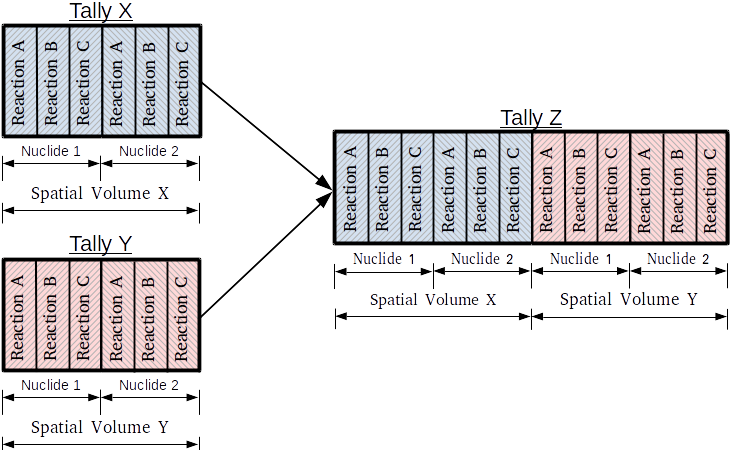
\includegraphics[width=\linewidth]{figures/workflow/openmc/tally-merge}
  \caption{}
\end{subfigure}
\begin{subfigure}{\textwidth}
  \centering
  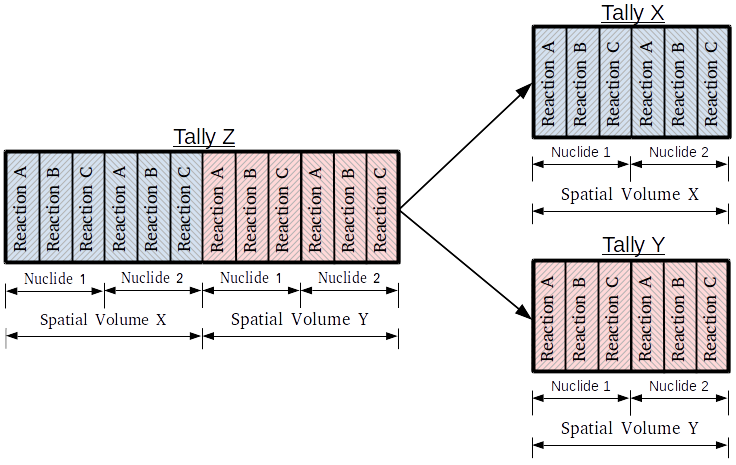
\includegraphics[width=\linewidth]{figures/workflow/openmc/tally-slice}
  \caption{}
\end{subfigure}
\caption[Tally merging and slicing operations]{Two \texttt{Tally} objects for different spatial volumes are merged into a single \texttt{Tally} (a). A single \texttt{Tally} is sliced by spatial volume into two distinct \texttt{Tally} objects (b).}
\label{fig:tally-merge-slice}
\end{figure}

%paragraph: aggregation (slicing/merging)
%-operations use NumPy to efficiently create derived sliced/merged tallies
%-slicing/merging can be used to slice tallies apart by nuclide, group, domain, etc.
%  -use tally merging to re-assembly MGXS from outputs of ML algorithms

%%%%%%%%%%%%%%%%%%%%%%%%%%%%%%%%
\subsubsection{Tally Arithmetic}
\label{subsubsec:chap4-tally-arithmetic}

As discussed in Sec.~\ref{subsec:chap3-tally-types}, a variety of reaction rate and flux tallies must be arithmetically combined in order to compute \ac{MGXS} with Monte Carlo (see Sec.~\ref{subsec:chap3-tally-types}). At the most general level, a reaction rate tally must be divided by a flux tally for each energy group, nuclide and tally volume (see Eqn.~\ref{eqn:chap3-general-micro}). In addition, the transport correction must be subtracted from the total cross section and scattering matrix (Eqns.~\ref{eqn:chap3-sigt-transport-macro} and~\ref{eqn:chap3-scatter-trans-macro}), and a summation must be performed over energy groups to compute the fission emission spectrum (Eqn.~\ref{eqn:chap3-chi}). Furthermore, it is desirable to compute a variance estimator for each \ac{MGXS} by propagating uncertainties as described in Sec.~\ref{subsec:chap3-uncertainty-prop}. The Python \ac{API} provides a novel feature known as \textit{tally arithmetic} to enable arithmetic combinations of tallies with efficient vectorized numerical operations across energy groups, nuclides and spatial tally zones.

Tally arithmetic is an object-oriented data processing feature which arithmetically combines two or more tallies and/or scalar values into new \textit{derived tallies}. The objective of tally arithmetic is to rapidly transform tally data with automated uncertainty propagation. The tally arithmetic implementation in OpenMC overloads the operators for addition, subtraction, multiplication, division, and exponentiation in the Python \ac{API}'s \texttt{Tally} class. In addition, the \texttt{Tally} class supports summation or averaging operations across some or all of its filter, nuclide or score bins.  The derived tallies produced from tally arithmetic provide the same rich functionality available for the \texttt{Tally} operands used in the arithmetic operation (\textit{e.g.}, Pandas DataFrames, tally arithmetic).

Multi-group cross sections may be simply and efficiently computed with tally arithmetic. For example, the following code snippet illustrates how tally slicing and arithmetic are used to compute a total \ac{MGXS}:

\lstinputlisting[language=Python, basicstyle=\ttfamily\footnotesize, caption={\ac{MGXS} calculation with tally arithmetic.}, label={lst:python-input}]{listings/workflow/tally-arithmetic.py}

\noindent The total \ac{MGXS} that is returned from the tally division operation is encapsulated within a \texttt{Tally} class. This is the approach used by the \ac{MGXS} generation module created for OpenMC in Sec.~\ref{subsec:chap4-mgxs}.

It should be noted that the uncertainty propagation in tally arithmetic makes the assumption that tallies represent independent random variables (see Sec.~\ref{subsec:chap3-uncertainty-prop}). However, in many if not most cases this assumption is untrue as tallies may be highly correlated. For example, there is a strong correlation between the flux and reaction rate tallies across the same material or cell, but this is not accounted for when these tallies are combined to compute \ac{MGXS} with tally arithmetic. In the future it may be possible to improve this approximation with the inclusion of tally covariance matrices in tally arithmetic.

%%%%%%%%%%%%%%%%%%%%%%%%%%%%%%%%%%%%%
\subsection{Distributed Cell Tallies}
\label{subsec:chap4-distribcells}

Many Monte Carlo codes, including OpenMC, use some variant of combinatorial geometry. because it can represent arbitrary, repeating geometries such as fuel pins and assemblies. However, the \ac{CG} approach is challenged by applications which require tallies in each instance of a repeated cell throughout a reactor geometry, such as the \ac{BEAVRS} benchmark model~\cite{horelik2013beavrs} depicted in Fig.~\ref{fig:beavrs}. The ``brute force'' solution is to instantiate a unique cell for each distinct tally zone. However, this defeats the purpose of using \ac{CG} for its compact representation, and it is not scalable to problems with large tally datasets such as those considered in this thesis.

\begin{figure}[h!]
  \centering
  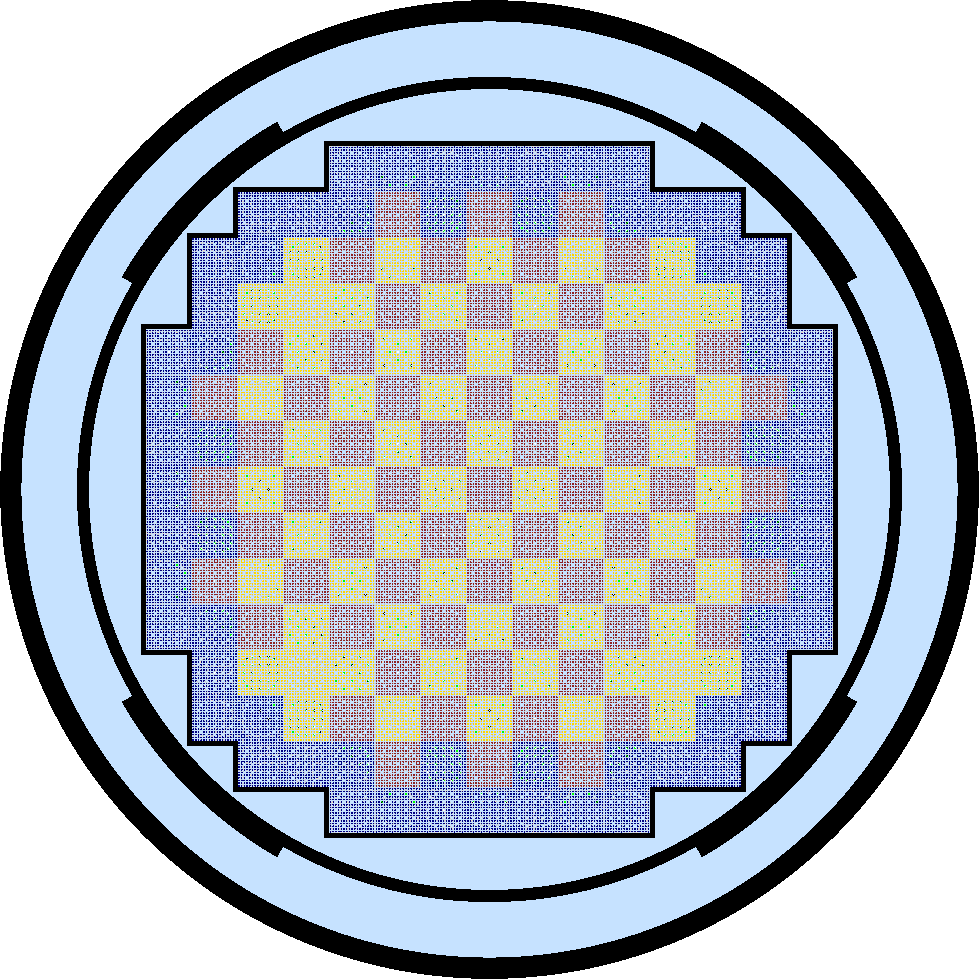
\includegraphics[width=2.5in]{figures/workflow/openmc/core}\hspace{1cm}
  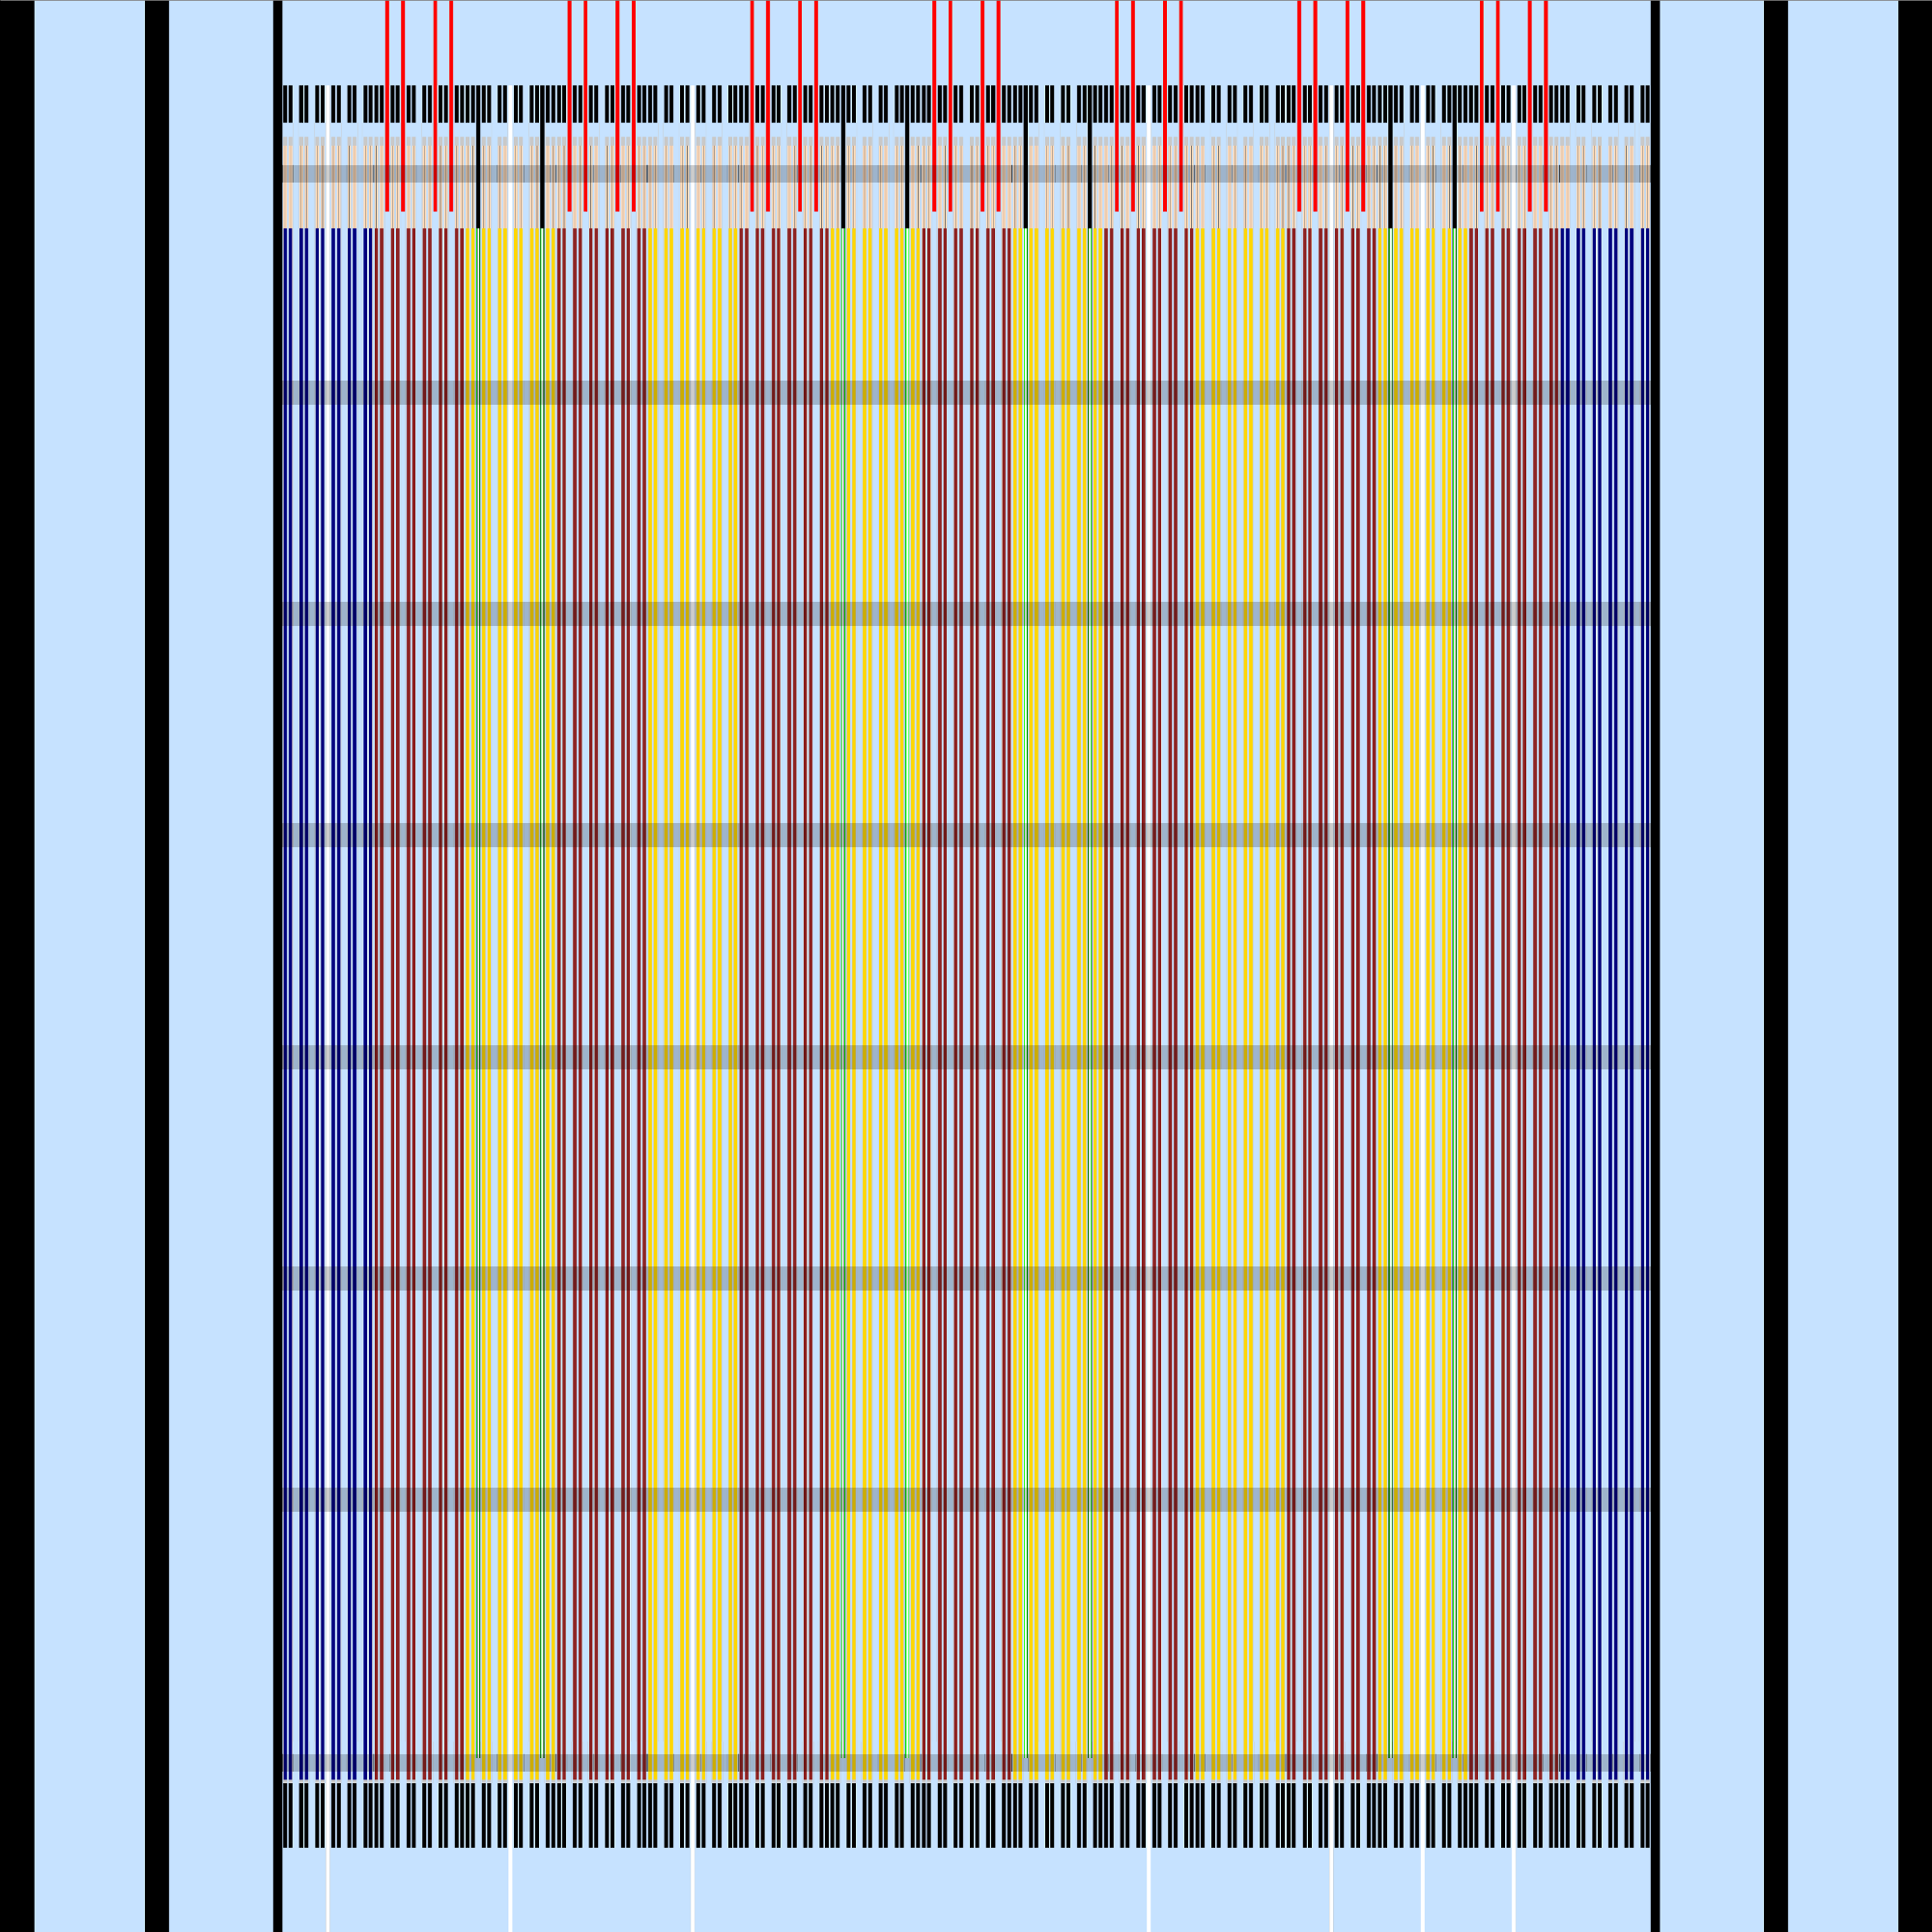
\includegraphics[width=2.5in]{figures/workflow/openmc/core_axial}
\caption[Radial and axial views of the BEAVRS core]{The radial (a) and axial (b) views of the BEAVRS \ac{PWR} core geometry~\cite{horelik2013beavrs}. The distributed cell tally algorithm provides a simple and efficient interface to tally within each of the 50,000+ fuel, guide tube, and burnable poison pin cells in complex heterogeneous models like the \ac{BEAVRS} core.}
\label{fig:beavrs}
\end{figure}

The \textit{distributed cell tally} algorithm was implemented in OpenMC to permit simply defined spatial tally zones across repeated cell instances~\cite{lax2014distribcell}. The distributed cell algorithm, commonly abbreviated as the \textit{distribcell} algorithm, classifies each unique cell instance using \textit{maps} and \textit{offsets} which consume orders of magnitude less memory than would be required by the ``brute force'' approach. Only a single transparent line of \ac{XML} input is necessary to define a distribcell tally which may span across an arbitrary number of instances for a particular cell. Furthermore, the Python \ac{API} may be used to perform efficient vectorized transformations of distribcell tally data stored as contiguous NumPy arrays. The distribcell tally algorithm was used to compute spatially-varying \ac{MGXS} across fuel pin cell instances for the spatial homogenization methology introduced in Chaps.~\Crefrange{chap:benchmarks}{chap:unsupervised}.

The distribcell tally algorithm consists of pre-processing and indexing stages. The pre-processing phase builds a mapping to index unique regions based on the unique combination of cells, universes and lattices used to construct each region. This is done by storing offset numbers in the data structures for each fill cell\footnote{Any cell that is filled with a nested universe or lattice of cells.}. The offset maps are recursively constructed starting from the top-level universe and proceeding through each lower nested universe level in the combinatorial geometry. The pre-processing algorithm tabulates the total number of instances of each cell in the geometry in order to dynamically allocate memory for distribcell tally arrays. At runtime, the on-the-fly indexing scheme efficiently computes cell instance IDs in order to index and score to the appropriate bin(s) in distribcell tallies. The cell instance IDs are simply found by summing the offsets at each nested universe level along the path to the cell instance in the \ac{CG} as shown in Fig.~\ref{fig:indexing-scheme}. The interested reader is referred to~\cite{lax2014distribcell} for more details about the distribcell tally algorithm, including pseudocode for both pre-processing and indexing, as well as a performance model for the memory footprint consumed by the offsets and maps.
  
\begin{figure}
  \centering
  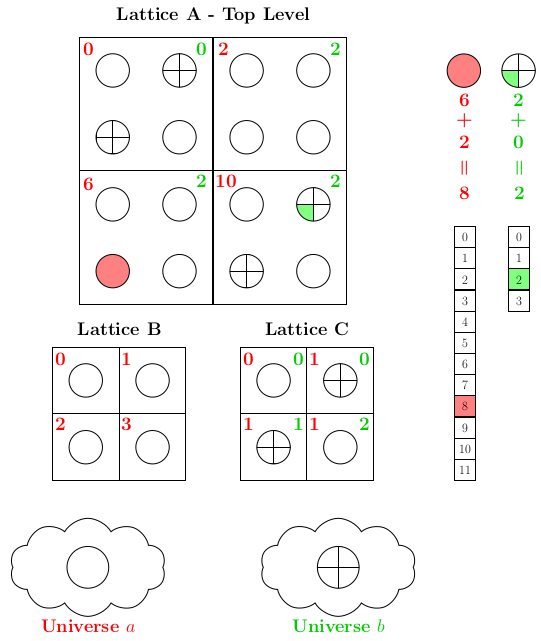
\includegraphics[width=\linewidth]{figures/workflow/openmc/distribcells}
\caption[The distributed cell tally indexing algorithm]{An example of the distribcell tally algorithm's on-the-fly indexing scheme~\cite{lax2014distribcell}. Material-filled cells are defined in pin cell universes $a$ and $b$, which are filled into the cells of lattices $B$ and $C$, which are filled into the cells of lattice $A$.  The colored numbers in each fill cell are the offsets for each base universe, which can be used to quickly compute a unique ID for each instance of a material cell.}
\label{fig:indexing-scheme}
\end{figure}

%%%%%%%%%%%%%%%%%%%%%%%%%%%%%%%%%%%%%%%%
\subsection{Isotropic in Lab Scattering}
\label{subsec:chap4-iso-in-lab}

As part of this thesis, a unique option for isotropic in lab scattering was implemented in the OpenMC code. The isotropic in lab (abbreviated as iso-in-lab) feature may be useful to quantify the ability of multi-group codes to capture anisotropic scattering effects with higher order scattering matrices or transport correction schemes (see Sec.~\ref{subsec:chap2-transport-corr}). The iso-in-lab scattering feature was implemented as a ``scattering'' attribute for each nuclide/element in a simulation. When iso-in-lab scattering is specified for a nuclide/element, the outgoing neutron energy is sampled from the scattering laws prescribed by the continuous energy cross section library, but the outgoing neutron direction of motion is sampled from an isotropic in lab distribution. 

Unless otherwise noted, isotropic in lab scattering was employed in OpenMC to generate the \ac{MGXS} used in this thesis. The iso-in-lab scattering feature enabled ``apples-to-apples'' comparisons between the reference eigenvalues and reaction rate distributions produced by OpenMC and those computed from isotropic multi-group calculations with OpenMOC.

%%%%%%%%%%%%%%%%%%%%%%%%%%%%
\subsection{MGXS Generation}
\label{subsec:chap4-mgxs}

The OpenMC Python \ac{API}'s \texttt{openmc.mgxs} module was implemented to generate multi-group cross sections. The \texttt{openmc.mgxs} module is built atop the underlying core features in the rest of the \ac{API} to support a seamless interface for both input generation and downstream data processing of \ac{MGXS} from Python. In particular, one may specify the \ac{MGXS} to compute and the \texttt{openmc.mgxs} module will construct the necessary \texttt{Tally} objects. The \texttt{Tally} objects may be easily exported to \ac{XML} input files for OpenMC, and used to containerize and process the tally data produced by an OpenMC simulation. The \texttt{openmc.mgxs} module thereby leverages the software stack of Pandas DataFrames, tally arithmetic, etc. provided by the OpenMC Python \ac{API}.

The \texttt{openmc.mgxs} module can compute macroscopic or microscopic \ac{MGXS} for individual nuclides or elements as well as collections of nuclides and elements\footnote{A \ac{MGXS} computed for a collection of nuclides/elements is the sum of the individual contributions from each nuclide/element.}. \ac{MGXS} can be computed in one or more arbitrary energy group structures. The module supports energy condensation in downstream data processing which is useful for exploring approximation bias in various energy group structures. For example, \ac{MGXS} may be computed in a 16-group structure and the tally data subsequently condensed to 2-group, 8-group, 12-group, etc. structures for multi-group calculations\footnote{Energy condensation may be performed to arbitrarily defined coarse group structures with \texttt{openmc.mgxs} provided the coarse group boundaries coincide with boundaries in the fine group structure.}. The analysis in this thesis computed \ac{MGXS} in the 70-group structure provided in Tab.~\ref{table:app-70-groups}, and condensed the \ac{MGXS} to the coarser group structures given in Appendix~\ref{app:energy-groups} as needed.

The \texttt{openmc.mgxs} module is designed to perform spatial homogenization on heterogeneous tally meshes for fine mesh transport codes. In OpenMC parlance, \ac{MGXS} may be computed for material, cell or universe spatial domains. In addition, the module supports \ac{MGXS} calculations for repeated cell instances using distribcell spatial tally domains (see Sec.~\ref{subsec:chap4-distribcells}). The \texttt{openmc.mgxs} module may also perform spatial homogenization on structured Cartesian tally meshes for coarse mesh multi-gropu calculations. This thesis computed \ac{MGXS} using distribcell tallies (\textit{e.g.}, \ac{MGXS} for each fuel pin instance in a geometry) to support the \ac{MGXS} spatial homogenization introduced in Chaps.~\Crefrange{chap:benchmarks}{chap:unsupervised}.

The \texttt{openmc.mgxs} module uses an object-oriented design based on an abstract \texttt{MGXS} class with subclasses for different reaction types. The \texttt{MGXS} subclasses are itemized in Tab.~\ref{table:chap4-mgxs-types} and compute multi-group constants from \ac{MC} tallies using the methods detailed in Sec.~\ref{subsec:chap3-tally-types}. It should be noted that some reaction types include variants which do or do not account for scattering multiplicity reactions (see Sec.~\ref{sec:chap2-scatt-prod}). For example, the transport correction used by the \texttt{TransportXS} class does not include $(n,xn)$ reactions while that employed by the \texttt{NuTransportXS} does account for scattering multiplicity. The \texttt{openmc.mgxs} module also includes a \texttt{Library} class which automates the construction of \texttt{MGXS} objects for different group structures, spatial domains, and reaction types.

\begin{table}[h!]
  \centering
  \caption[The MGXS types implemented for OpenMC]{The \ac{MGXS} types implemented by the \texttt{openmc.mgxs} module in OpenMC.}
  \small
  \label{table:chap4-mgxs-types} 
  \vspace{6pt}
  \begin{tabular}{l p{10cm}}
  \toprule
  \rowcolor{lightgray}
  {\bf Class} &
  {\bf Description} \\
  \midrule
  \texttt{TotalXS} & Total collision \\
  \texttt{TransportXS} & Transport-corrected total collision \\
  \texttt{NuTransportXS} & Transport-corrected total collision w/ scattering multiplicity \\
  \texttt{AbsorptionXS} & Absorption \\
  \texttt{CaptureXS} & Radiative capture \\
  \texttt{FissionXS} & Fission \\
  \texttt{NuFissionXS} & Fission production \\
  \texttt{KappaFissionXS} & Fission energy release \\
  \texttt{ScatterXS} & Scattering \\
  \texttt{NuScatterXS} & Scattering w/ scattering multiplicity \\
  \texttt{ScatterMatrixXS} & Scattering matrix \\
  \texttt{NuScatterMatrixXS} & Scattering matrix w/ scattering multiplicity \\
  \texttt{Chi} & Fission emission spectrum \\
  \texttt{ChiPrompt} & Prompt fission emission spectrum \\
  \bottomrule
\end{tabular}
\end{table}

The \texttt{openmc.mgxs} module was developed with general design principles to generate \ac{MGXS} for any multi-group neutron transport code. Although the module does not explicitly support any multi-group codes, it can export \ac{MGXS} data to a variety of data storage formats, including \ac{CSV} and \ac{HDF5}. The exported \ac{MGXS} files may be easily transformed into the database or input files required by a particular multi-group code. As discussed in the following section, this thesis developed a tightly integrated framework to pipeline \ac{MGXS} generated by \texttt{openmc.mgxs} into the multi-group OpenMOC code.


%%%%%%%%%%%%%%%%%%%%%%%%%%%%%%%%%%%%%%%%%%%%%%%%%%%%%%%%%%%%%%%%%%%%%%%%%%%%%%%%
\section{OpenMOC}
\label{sec:chap4-openmoc}

The OpenMOC code is a multi-group neutron transport code implementing the deterministic Method of Characteristics (MOC)~\cite{boyd2014openmoc}. OpenMOC was initially developed to support a series of M.S. theses at MIT~\cite{li2013ms,boyd2014ms,shaner2014ms} and was later released for public use with the MIT open source license. Although this thesis could have plausibly used any multi-group code, OpenMOC was chosen for its flexible Python interface, computationally efficient algorithms, and the author's familiarity with the open source codebase.

%-reference need for MG code to evaluate MGXS for this thesis

This thesis inspired the development of new features and extensions which have been incorporated into the official OpenMOC codebase. This section begins with a brief overview of the \ac{MOC} implementation in OpenMOC in Sec.~\ref{subsubsec:chap4-openmoc-overview}. Various improvements were made to the OpenMOC Python interface as discussed in Sec.~\ref{subsubsec:chap4-openmoc-python}, while Sec.~\ref{subsubsec:chap4-openmoc-mgxs} details a module created to interface with \ac{MGXS} generated by OpenMC. The parallel algorithms and numerical acceleration schemes in OpenMOC which were used by this thesis are mentioned in Secs.~\ref{subsubsec:chap4-openmoc-parallel} and~\ref{subsubsec:chap4-openmoc-cmfd}, respectively.

%-improvements to the parallelism, CMFD to enable ``multi-sim'' calculations

%%%%%%%%%%%%%%%%%%%%%%%%%%%%%%%%%
\subsection{Methods Overview}
\label{subsubsec:chap4-openmoc-overview}

The method of characteristics is a widely used technique for solving partial differential equations, including the Boltzmann form of the neutron transport equation~\cite{askew1972moc}. Although not a stochastic formulation, \ac{MOC} is a ray-based algorithm akin to Monte Carlo particle tracking-based methods. In contrast to Monte Carlo, \ac{MOC} uses a fixed angular quadrature that is determined \textit{a priori}. This quadrature is used to specify 1D characteristics that cross the spatial domain. Prior to the physics computation, ray tracing must be performed to subdivide each characteristic into segments within different regions in the spatial mesh. Fig.~\ref{fig:moc-model} illustrates the spatial mesh and cyclic characteristic laydown used by the OpenMOC code.

\ac{MOC} propagates the angular neutron flux along each characteristic through each spatial zone. For each segment, the angular flux is attenuated due to neutron absorption and enhanced due to neutron fission or scattering in the corresponding spatial zone. \ac{MOC} uses the multi-group energy approximation such that this computation is performed for neutrons within discretized energy groups (see Sec.~\ref{subsec:chap2-energy}). Finally, an angular quadrature is applied to combine the average angular flux contribution from each characteristic to compute the average scalar flux in each zone and energy group.

\begin{figure}[h!]
  \begin{subfigure}[htb!]{0.32\textwidth}
    \centering
    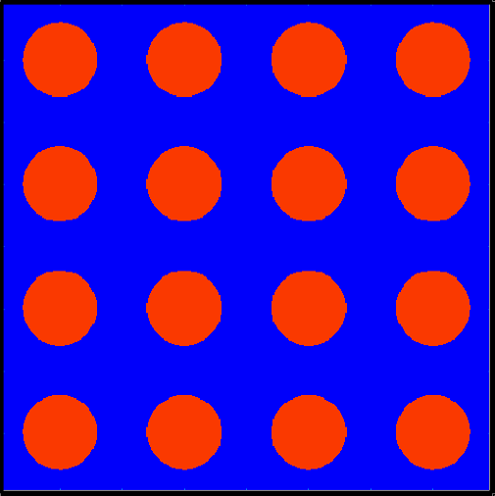
\includegraphics[width=0.95\textwidth]{figures/workflow/openmoc/materials-border}
    \label{fig:moc-model-materials}
    \caption{}
  \end{subfigure}
  \begin{subfigure}[htb!]{0.32\textwidth}
    \centering
    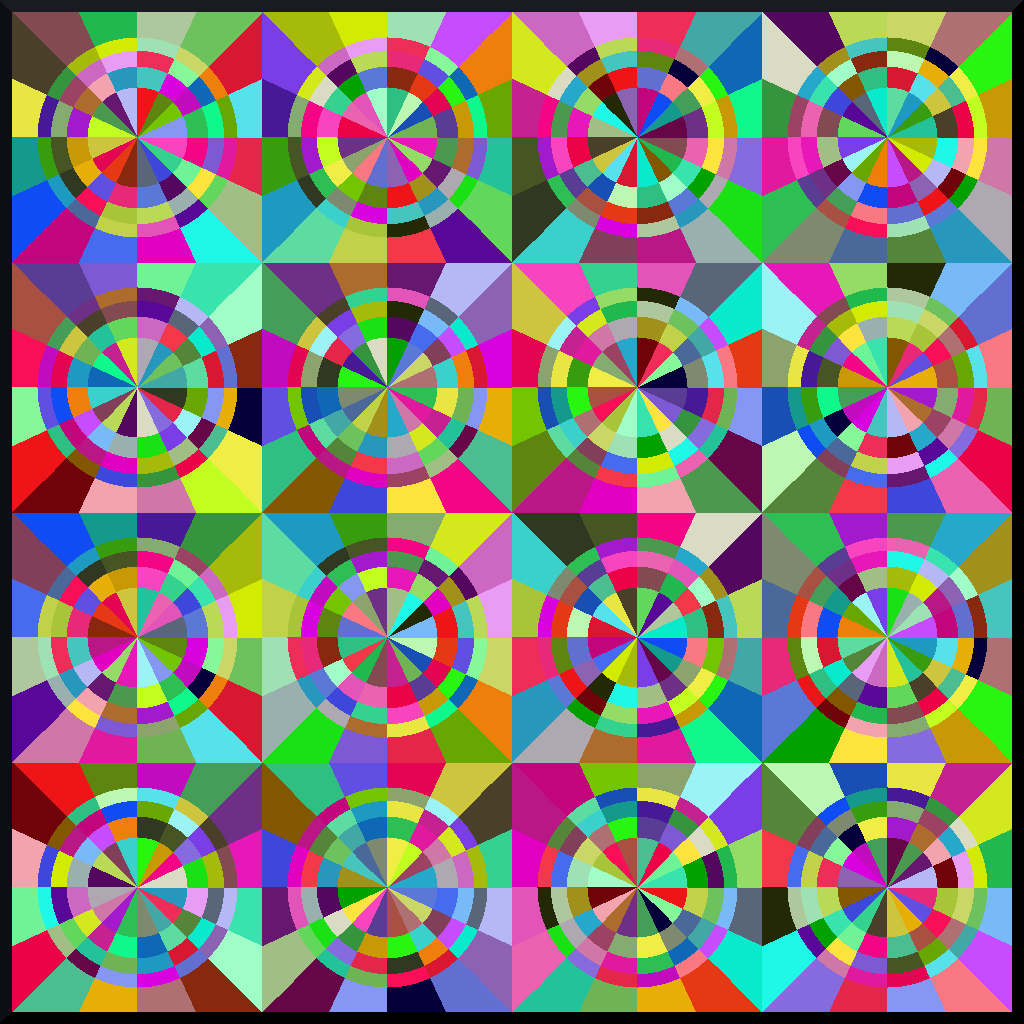
\includegraphics[width=0.95\textwidth]{figures/workflow/openmoc/FSRs}
    \label{fig:moc-model-fsrs}
    \caption{}
  \end{subfigure}
  \begin{subfigure}[htb!]{0.32\textwidth}
    \centering
    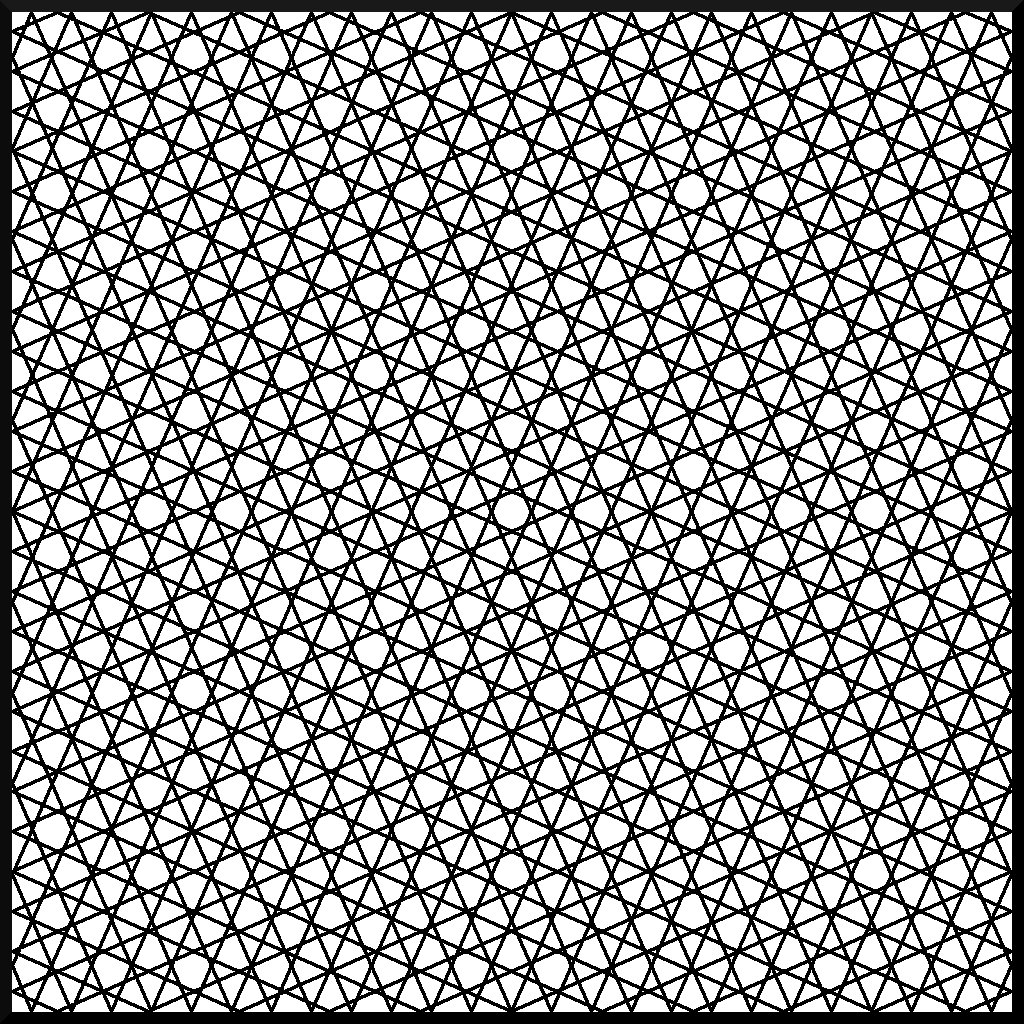
\includegraphics[width=0.95\textwidth]{figures/workflow/openmoc/cyclic-tracks}
    \label{fig:moc-model-tracks}
    \caption{}
  \end{subfigure}
\caption[Example OpenMOC flat source region mesh and track laydown]{The coolant and fuel materials (a), flat source region spatial mesh (b), and cyclic characteristic laydown (c) for a 4 $\times$ 4 fuel pin lattice taken from~\cite{boyd2016parallel}.}
\label{fig:moc-model}
\end{figure}

The OpenMOC code is capable of performing 2D \ac{MOC} calculations for light water reactor core configurations. OpenMOC discretizes the 2D geometry into flat source regions (FSRs) which approximate the neutron source as constant across each spatial zone\footnote{The neutron source may include any combination of fission, scattering and fixed sources.}. Furthermore, OpenMOC approximates the scattering source as isotropic in the lab coordinate system and is not yet able to use higher order scattering moment matrices. OpenMOC uses a power iteration scheme to solve for the dominant eigenvalue and eigenvector in criticality calculations. As part of this thesis, a general purpose fixed source solver was implemented to enable the detailed investigation of approximation bias in \ac{MGXS} as discussed in Chap.~\ref{chap:sph}. The interested reader is referred to the online code manual~\cite{openmoc2016manual} for more information detailing the \ac{MOC} implementation in OpenMOC.

%%%%%%%%%%%%%%%%%%%%%%%%%%%%%%%%%
\subsection{Python Interface}
\label{subsubsec:chap4-openmoc-python}

One of the key reasons that OpenMOC was used by this thesis was to leverage its flexible Python interface. The majority of the source code is written in C++ using object-oriented software design principles. The \ac{SWIG}~\cite{beazley2003swig} is deployed to expose the C++ classes and routines to the Python scripting language. The Python interface made it possible to tightly couple OpenMOC with the rich ecosystem of Python-based data processing and visualization tools for the spatial homogenization methodology developed in Chaps.~\Crefrange{chap:benchmarks}{chap:unsupervised}.

As part of this work, a new scheme was implemented to efficiently link OpenMOC's Python and C++ \ac{CG} data structures into a hierarchical tree-like data structure. This made it possible to use the OpenCG region differentiation algorithm discussed in Sec.~\ref{sec:chap4-region-diff} to derive geometries for OpenMOC. In addition, a thread-safe memory management model was realized which unifies the dynamic deallocation of objects shared between Python and C++ code. The memory model enabled 100s of OpenMOC simulations to be orchestrated by Python for the parametric studies considered in this thesis.

%\begin{figure}[h!]
%  \centering
%  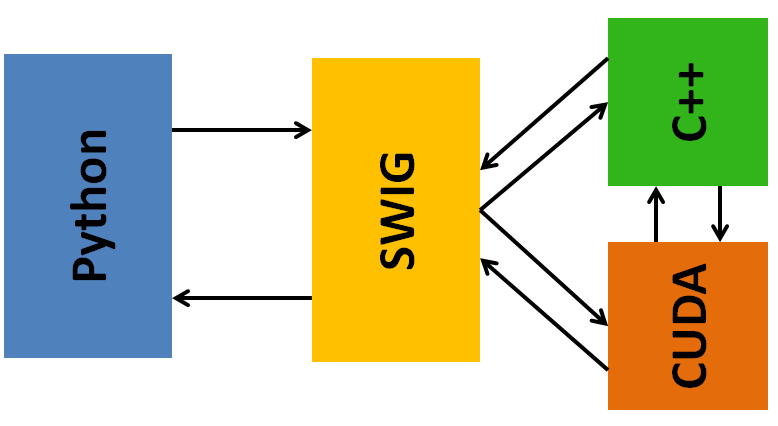
\includegraphics[width=0.7\linewidth]{figures/workflow/openmoc/software-design}
%\caption[The OpenMOC programming model]{The programming model used by OpenMOC to couple compiled C/C++/CUDA code to the Python interface using \ac{SWIG} taken from~\cite{boyd2014openmoc}.}
%\label{fig:openmoc-swig}
%\end{figure}

%%%%%%%%%%%%%%%%%%%%%%%%%%%%%%%%%
\subsection{Multi-Group Cross Sections}
\label{subsubsec:chap4-openmoc-mgxs}

OpenMOC uses multi-group macroscopic nuclear cross sections specified in any arbitrary energy group structure. Isotropic concentrations are not used since OpenMOC does not perform self-shielding or depletion calculations. Multi-group cross sections may be specified for each material or cell in the \ac{CG} used in a simulation. OpenMOC requires total, fission production and scattering matrix cross sections along with a fission emission spectrum\footnote{Transport-corrected total cross sections and scattering matrices may be used in OpenMOC.}. In addition, a fission cross section may be optionally supplied in order to compute spatially-varying fission reaction rates.

Cross section data is encapsulated by the \texttt{Material} class. A \texttt{Material} object may be instantiated in Python and cross section data loaded into it from NumPy arrays~\cite{walt2011numpy}. For simulations with many different materials (such as those in this thesis), defining nuclear cross section data by hand in a Python script is cumbersome and error prone. In order to minimize this painstaking process, the \texttt{openmoc.materialize} module was implemented to automate the loading \ac{MGXS} data into OpenMOC \texttt{Material} objects. This module can either import \ac{MGXS} data from HDF5 binary files~\cite{koranne2011hdf5} or extract \ac{MGXS} data from OpenMC \texttt{Library} Python objects (see Sec.~\ref{subsec:chap4-mgxs}). The \texttt{openmoc.materialize} module is designed to support large \ac{MGXS} libraries such as those produced from the spatial homogenization methodology introduced in Chaps.~\Crefrange{chap:benchmarks}{chap:unsupervised}. In addition, a scheme to compute \ac{SPH} factors to ensure reaction rate consistency with OpenMC was implemented in \texttt{openmoc.materialize} and is discussed in detail in Chap.~\ref{chap:sph}.

%%%%%%%%%%%%%%%%%%%%%%%%%%%%%%%%%
\subsection{Parallelism}
\label{subsubsec:chap4-openmoc-parallel}

OpenMOC's high performance parallel solvers for both multi-core \ac{CPUs} and \ac{GPUs} were extensively used for the analyses presented in this thesis. A shared memory parallel solver implemented in C++ using OpenMP~\cite{openmp2013} has demonstrated excellent scalability on a range of multi-core architectures\cite{boyd2016parallel}. In addition, OpenMOC includes a highly parallel implementation which uses the CUDA programming language~\cite{nvidia2012cuda} to run on NVIDIA \ac{GPUs} with 100s to 1000s of lightweight cores~\cite{boyd2013massively}. OpenMOC's parallel solvers made it possible to perform large parametric studies of 100s of \ac{MOC} simulations to evaluate the spatial homogenization methodology introduced in Chaps.~\Crefrange{chap:benchmarks}{chap:unsupervised}.


%%%%%%%%%%%%%%%%%%%%%%%%%%%%%%%%%
\subsection{CMFD Accleration}
\label{subsubsec:chap4-openmoc-cmfd}

OpenMOC uses the Coarse Mesh Finite Difference (CMFD) acceleration scheme to greatly reduce the number of iterations required to converge criticality calculations~\cite{boyd2014openmoc}. \ac{CMFD} acceleration functions by using the solution of a coarse mesh diffusion problem to accelerate the convergence of the fine mesh \ac{MOC} transport problem. The details of the \ac{CMFD} implementation in OpenMOC are beyond the scope of this thesis, and the interested reader is referred to the online code manual~\cite{openmoc2016manual} for more information. 

\ac{CMFD} acceleration was extensively used to accelerate the eigenvalue calculations in this thesis. All simulations which employed \ac{CMFD} used the novel $k$-Nearest Neighbors prolongation scheme created by Shaner~\cite{shaner2015cmfd} and implemented in OpenMOC to improve the convergence rate and stability of \ac{CMFD}. In particular, all simulations used three neighbors along with a successive over-relaxation (SOR) factor of unity. Along with OpenMOC's parallel solvers, \ac{CMFD} acceleration made it feasible to perform large parametric studies to generate the results presented in this thesis.

%\begin{figure}[h!]
%  \centering
%  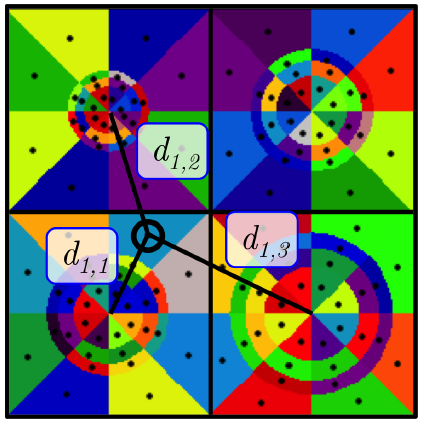
\includegraphics[width=0.5\linewidth]{figures/workflow/openmoc/centroid}
%\caption[$k$-nearest neighbor centroid scheme for CMFD]{The $k$-nearest neighbor centroid update scheme for \ac{CMFD}~\cite{shaner2015cmfd}.}
%\label{fig:knn-cmfd}
%\end{figure}


%%%%%%%%%%%%%%%%%%%%%%%%%%%%%%%%%%%%%%%%%%%%%%%%%%%%%%%%%%%%%%%%%%%%%%%%%%%%%%%%
\section{OpenCG}
\label{sec:chap4-opencg}

The OpenCG code~\cite{boyd2015opencg} was created to simplify the process of creating and transferring data mapped to combinatorial geometries for OpenMC and OpenMOC. Combinatorial geometry\footnote{\ac{CG} is often referred to as constructive solid geometry in the neutron transport literature.} is commonly used by neutron transport simulation codes since it:

\begin{itemize}[noitemsep]
  \item Permits description of an \textit{arbitrarily accurate} unstructured geometric mesh
  \item Provides a \textit{compact representation} with minimal input description
  \item Represents $\mathcal{O}(n)$ components with $\mathcal{O}(\log{}n)$ memory requirements
  \item Utilizes a hierarchical \textit{tree data structure} with scalable $\mathcal{O}(\log{}n)$ traversals
\end{itemize}

\noindent Although many codes utilize \ac{CG}, it is overly burdensome to manually write geometric input files for multiple simulation tools for code verification of a single reactor model. In addition, the compact geometric representation is not well-suited for large scale analysis of spatially-varying data in nuclear reactor cores -- such as distributed cell tally data in OpenMC -- without new algorithms to guide and automate the process. This thesis developed a new \ac{CG} modeling tool called OpenCG to accelerate the building of complicated reactor geometries, enable rapid cross-code verification and facilitate large scale data processing. 

OpenCG is a simple-to-use Python library which may be used to construct a single geometry for use in both OpenMC and OpenMOC. In addition, OpenCG enables data transfer between OpenMC and OpenMOC as illustrated in Fig.~\ref{fig:chap4-simulation-triad}. In particular, OpenCG accomodates the generation of \ac{MGXS} from distributed cell tallies on OpenMC's \ac{CG} mesh and maps them to the flat source region spatial mesh used by OpenMOC. A variant of OpenMC's distributed cell tally algorithm (see Sec.~\ref{subsec:chap4-distribcells}) was implemented in OpenCG to make this possible. In addition to transferring \ac{MGXS} data, OpenCG enabled the comparison of pin-wise reaction rate distributions computed from OpenMC distribcell tallies with those computed on OpenMOC's \ac{FSR} mesh.

The following sections outline the key features implemented in OpenCG for this thesis and follows a recent paper by this author~\cite{boyd2015opencg}. Sec.~\ref{sec:chap4-opencg-compatibility} discusses the compatibility modules which tie OpenCG, OpenMC and OpenMOC into a simulation triad. In addition, two novel algorithms known as \ac{LNS} and region differentiation were developed in OpenCG to enable the spatial homogenization methodology introduced in this thesis, and are presented in Secs.~\ref{sec:chap4-lns} and~\ref{sec:chap4-region-diff}, respectively.

%%%%%%%%%%%%%%%%%%%%%%%%%%%%%%%%%%%%
\subsection{Compatiblity Modules}
\label{sec:chap4-opencg-compatibility}

The simulation triad of OpenCG, OpenMC and OpenMOC shown in Fig.~\ref{fig:chap4-simulation-triad} is made possible with compatibility modules. The compatibility modules allow the construction of a single geometry using OpenCG's Python \ac{CG} primitives for surfaces, cells, universes and lattices. The OpenCG geometry may then be exported to OpenMC or OpenMOC using compatibility modules developed for each code.

For example, OpenMC includes a Python \ac{API} with object-oriented \ac{CG} primitives. This \ac{API}'s primitives include routines to directly export themselves to the \ac{XML} input file format used by OpenMC. The OpenCG-OpenMC compatibility module allows OpenCG's primitives to be transformed into the corollaries within the OpenMC Python \ac{API}, and vice versa. Likewise, the OpenCG-OpenMOC compatibility module allows OpenCG's primitives to be transformed into the corollaries within the OpenMOC Python/C++ code. In summary, the compatibility modules enable the rapid, automated exportation of various OpenCG geometries directly to OpenMC and OpenMOC.

OpenCG's object-oriented Python software model permits greater freedom for geometric parameter optimization than can be easily achieved with traditional \ac{ASCII} or \ac{XML} input files. In particular, the compatibility module framework enabled a dynamic workflow between OpenMC and OpenMOC for \ac{MGXS} generation and code verification in this thesis. For example, OpenCG's region differentiation algorithm (see Sec.~\ref{sec:chap4-region-diff}) was used to produce 100s of geometries composed with different \ac{MGXS} libraries to evaluate the spatial homogenization methodology introduced in Chaps.~\Crefrange{chap:benchmarks}{chap:unsupervised}.

%\begin{figure}[h!]
%  \centering
%  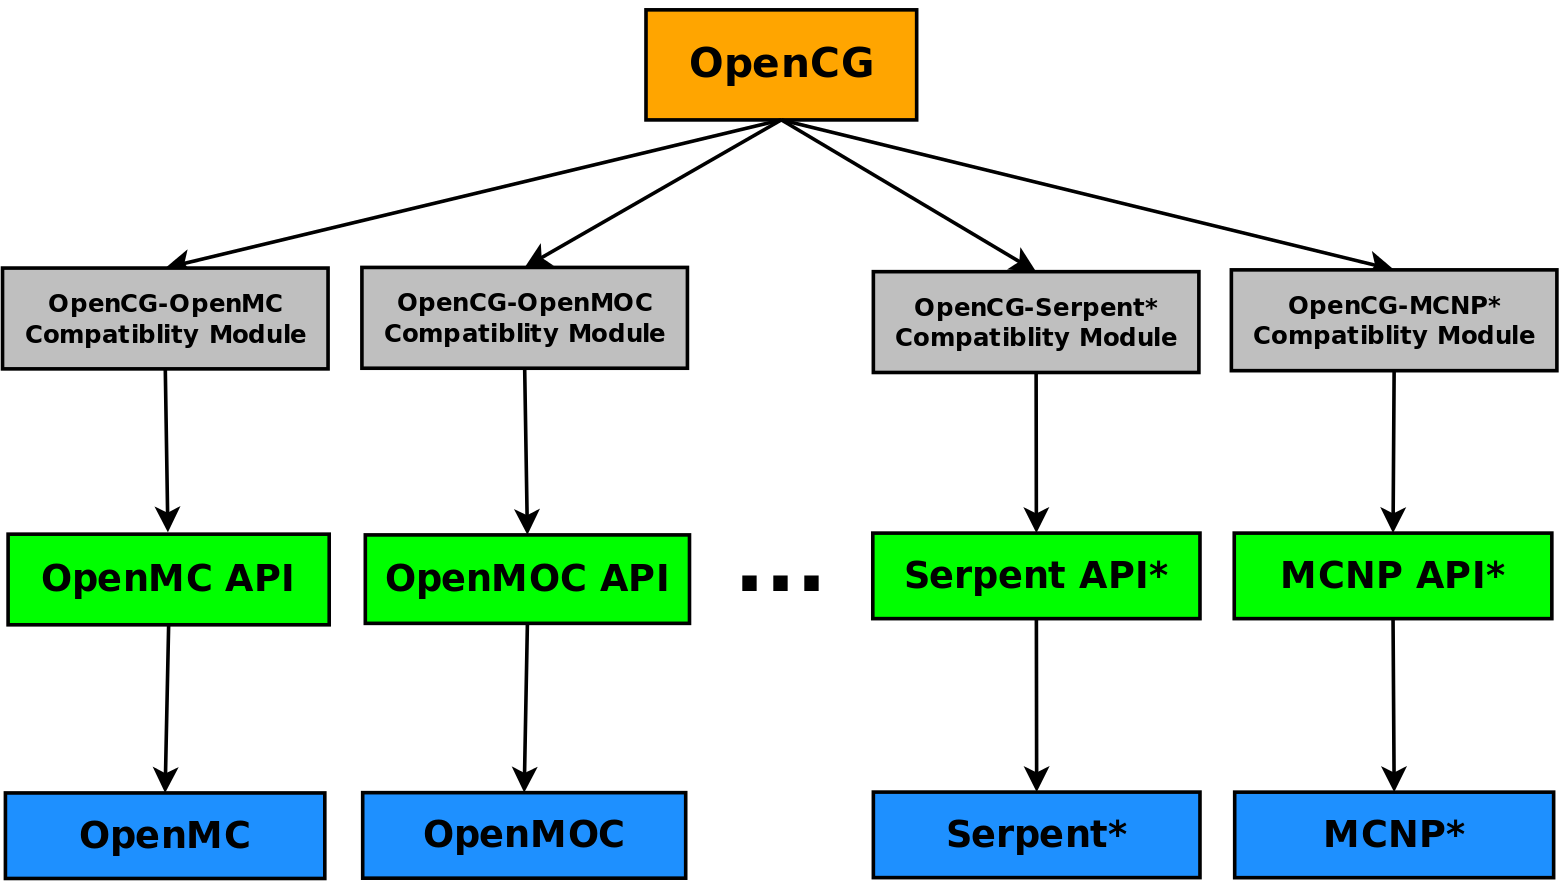
\includegraphics[width=.8\linewidth]{figures/workflow/opencg/compatibility-modules}
%  \caption{OpenCG compatibility modules for various neutron transport codes. The compatibility modules for OpenMC and OpenMOC will be released in future public distributions of each code, while modules for Serpent and MCNP are in progress at the time of this writing.}
%  \label{fig:compatibility-modules}
%\end{figure}


%%%%%%%%%%%%%%%%%%%%%%%%%%%%%%%%%%%%
\subsection{Local Neighbor Symmetry}
\label{sec:chap4-lns}

One of the unique algorithms implemented in OpenCG explicitly for this thesis is known as Local Neighbor Symmetry (LNS) identification~\cite{boyd2015opencg}. The LNS algorithm is motivated by this thesis' objective to accurately predict spatial zones that experience similar spectral self-shielding effects. The \ac{LNS} algorithm performs a systematic analysis of a \ac{CG} tree data structure to identify neighbor cells, or pairs of cells which are adjacent to one another. The neighbor cells are assembled into a heuristic which groups like spatial zones with common \ac{LNS} identifiers. The \ac{LNS} algorithm is analogous to the geometric templates used in lattice physics codes such as CASMO~\cite{edenius1995casmo} to identify fuel pins which have similar \ac{MGXS} in a fuel assembly.

The \ac{LNS} algorithm identifies the unique symmetry for the path to a region in a combinatorial geometry as described in Alg.~\ref{alg:local-neighbor-symmetry-cells}. \ac{LNS} performs a \ac{BFS} to find neighbors on each level of the \ac{CG} tree. For example, \ac{BFS} is used to find neighbor cells for a particular cell within a universe. Similarly, \ac{BFS} is used to find neighbor universes adjacent to a particular lattice cell. The neighbor cells and universes on each of the $k$ levels of a \ac{CG} tree are connected to form a $k$-partite graph\footnote{A $k$-partite graph is a graph whose graph vertices can be partitioned into $k$ disjoint sets so that no two vertices within the same set are adjacent~\cite{weisstein2012kpartite}.} as depicted in Fig.~\ref{fig:lns-k-partite-graph}. Finally, the $k$-partite graph is used as an argument to a hash function to compute the \ac{LNS} identifier (\textit{e.g}, a non-negative integer) for the particular region represented by the path. This algorithmic formulation is general to any arbitrary combinatorial geometry, including those commonly used to model \ac{LWRs} with nested rectilinear lattices.

\begin{algorithm}[h!]
\caption[OpenCG's Local Neighbor Symmetry Identification]{Local Neighbor Symmetry Identification}
\label{alg:local-neighbor-symmetry-cells}
\begin{algorithmic}[1]
\Procedure{computeNeighborSymmetry}{$path$}
    \State $G \gets \emptyset$ \Comment{Initialize empty set for graph}
    \State $k \gets$ \textbf{length}($path$) \Comment{Find number of independent sets}
    \For{$i := 1, k$}
        \If{\textbf{type}($path[i]$) \textbf{is} UNIVERSE}
            \State $G \gets G \cup \{path[i]\}$ \Comment{Append universe to graph}
        \ElsIf{\textbf{type}($path[i]$) \textbf{is} LATTICE}
            \State $N \gets$ \Call{BreadthFirstSearch}{$path[i]$} \Comment{Find lattice cell neighbors}
            \State $G \gets G \cup \{N\}$ \Comment{Append neighbors to graph}
        \ElsIf{\textbf{type}($path[i]$) \textbf{is} CELL}
            \State $N \gets$ \Call{BreadthFirstSearch}{$path[i]$} \Comment{Find cell neighbors}
            \State $G \gets G \cup \{N\}$ \Comment{Append neighbors to graph}
        \EndIf
    \EndFor
    \State \textbf{return} \Call{Hash}{$G$} \Comment{Return $k$-partite graph hash}
\EndProcedure
\end{algorithmic}
\end{algorithm}

\begin{figure}[h!]
  \centering
  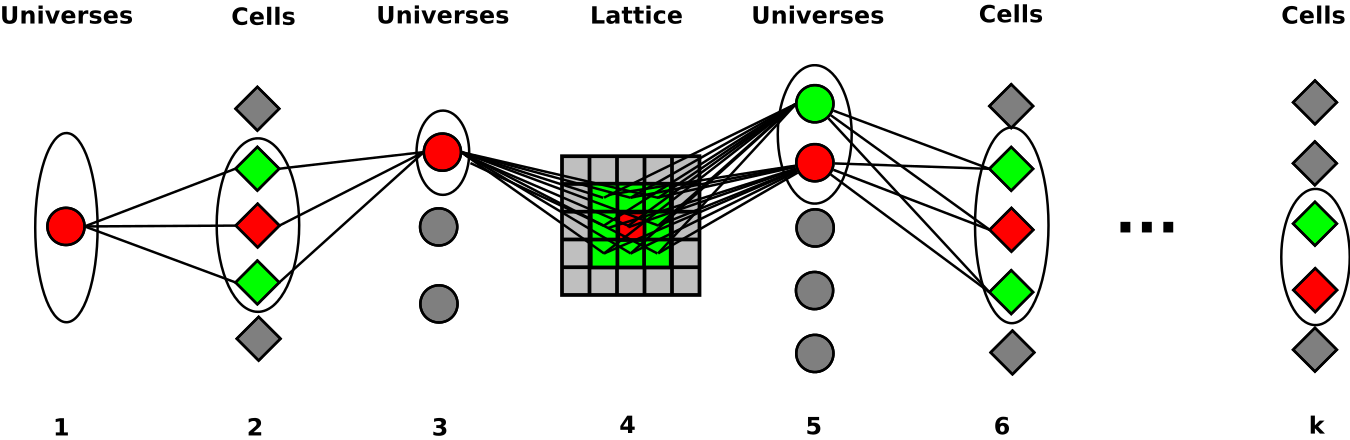
\includegraphics[width=\linewidth]{figures/workflow/opencg/neighbors-k-partite-graph}
  \caption[A $k$-partite graph created by the OpenCG LNS algorithm]{An example $k$-partite graph structure used to identify local neighbor symmetries. Red nodes correspond to the universes/cells encapsulating a region of interest, green nodes correspond to the neighbors of that region, and gray nodes correspond to universes/cells which are not neighbors. Red and green nodes at each level are combined into an argument for a hash function to generate a \ac{LNS} ID for the region of interest.}
  \label{fig:lns-k-partite-graph}
\end{figure}

Several parameters are incorporated into OpenCG's \ac{LNS} \ac{API} to provide the user with various methods to adjust the number of symmetries discovered by the algorithm. For example, OpenCG includes \textit{general} and \textit{unique} neighbor identifiers. General neighbors includes all neighbor cells/universes found by \ac{BFS} -- including duplicates -- as separate nodes in the $k$-partite graph. For example, a single universe may be placed multiple times around a lattice cell, each instance of which will be independently discovered by \ac{BFS} and replicated as a distinct node within the graph. On the contrary, unique neighbors does not include duplicate cells/universes -- only unique cells/universes are represented by distinct nodes in each independent set in the $k$-partite graph. A few diagrams of general and unique \ac{LNS} applied to two geometries are depicted in Fig.~\ref{fig:neighbor-cells}.

\begin{figure}[h!]
\begin{subfigure}{.5\textwidth}
  \centering
  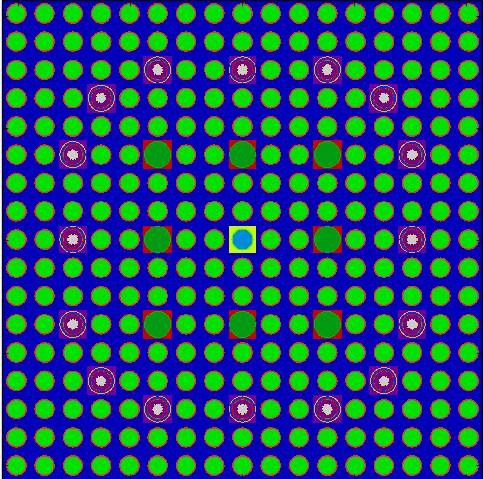
\includegraphics[width=.7\linewidth]{figures/workflow/opencg/cells-xy-24-16-assm}
  \caption{}
  \label{fig:assm-cells}
\end{subfigure}%
\begin{subfigure}{.5\textwidth}
  \centering
  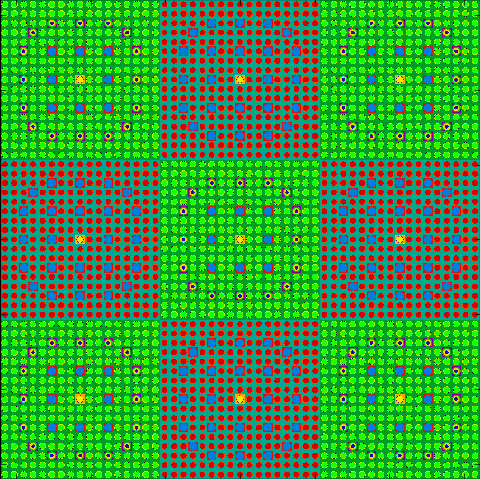
\includegraphics[width=.7\linewidth]{figures/workflow/opencg/cells-xy-colorset}
  \caption{}
  \label{fig:colorset-cells}
\end{subfigure}
\begin{subfigure}{.5\textwidth}
  \centering
  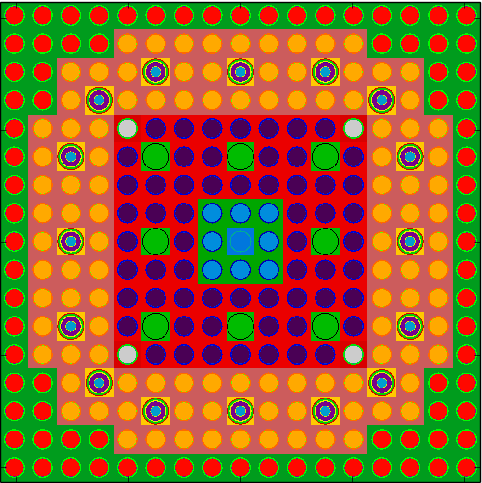
\includegraphics[width=.7\linewidth]{figures/workflow/opencg/unique-neighbor-cells-xy-24-16-assm}
  \caption{}
  \label{fig:assm-unique-neighbors}
\end{subfigure}
\begin{subfigure}{.5\textwidth}
  \centering
  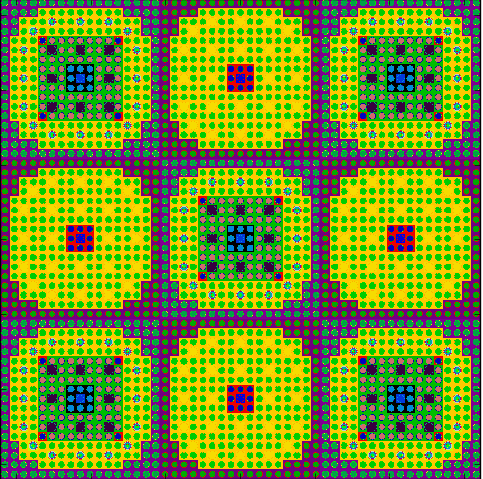
\includegraphics[width=.7\linewidth]{figures/workflow/opencg/unique-neighbor-cells-xy-colorset}
  \caption{}
  \label{fig:colorset-unique-neighbors}
\end{subfigure}
\begin{subfigure}{.5\textwidth}
  \centering
  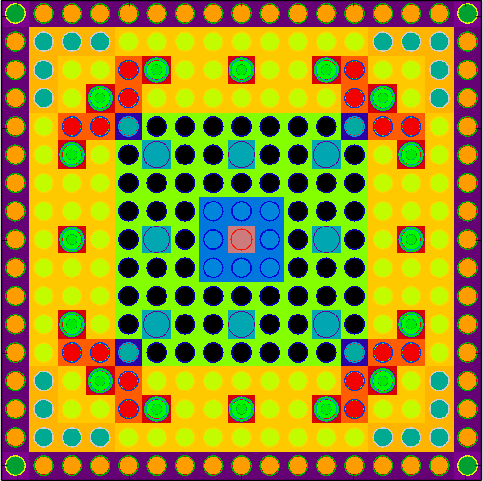
\includegraphics[width=.7\linewidth]{figures/workflow/opencg/neighbor-cells-xy-24-16-assm}
  \caption{}
  \label{fig:assm-neighbors}
\end{subfigure}
\begin{subfigure}{.5\textwidth}
  \centering
  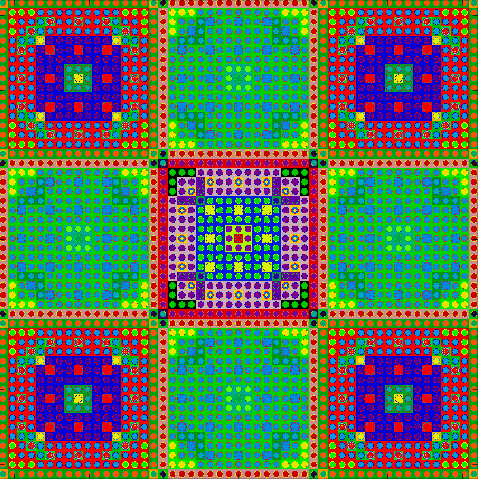
\includegraphics[width=.7\linewidth]{figures/workflow/opencg/neighbor-cells-xy-colorset}
  \caption{}
  \label{fig:colorset-neighbors}
\end{subfigure}
\caption[Example OpenCG Local Neighbor Symmetry mappings]{Two rectilinear lattice geometries are depicted to illustrate the use of local neighbor symmetry identification~\cite{boyd2015opencg}. The \textit{cells} are depicted for (a) a 17$\times$17 PWR lattice and (b) a 3$\times$3 colorset of two different 17 $\times$ 17 PWR assemblies each with burnable absorbers, guide tubes and instrument tubes. The \textit{unique neighbor} symmetry identifiers are color-coded in (b) and (c) for the assembly and colorset, respectively. Likewise, the \textit{general neighbor} symmetry identifiers are color-coded in (d) and (f).}
\label{fig:neighbor-cells}
\end{figure}

To this author's knowledge there is no other implementation of \ac{LNS} aside from that in the OpenCG code. The \ac{LNS} algorithm was used extensively in this thesis as a deterministic ``clustering'' technique for the spatial homogenization methodology introduced in Chaps.~\Crefrange{chap:benchmarks}{chap:unsupervised}. In particular, \ac{LNS} was used to predict which fuel pins have similar \ac{MGXS} in \ac{LWRs} due to spatial self-shielding effects induced by neighboring fuel, guide tube and absorber pins. The \ac{LNS} scheme served as a proxy to the traditional geometric template approach used in lattice physics codes to group pins with like \ac{MGXS}. The spatial homogenization methodology developed in Chaps.~\Crefrange{chap:benchmarks}{chap:unsupervised} incorporates \ac{MC} tally data in unsupervised clustering in an attempt to outperform \ac{LNS}' analysis based solely on the geometry.


%%%%%%%%%%%%%%%%%%%%%%%%%%%%%%%%%%%%
\subsection{Region Differentiation}
\label{sec:chap4-region-diff}

As previously noted, one of the advantages of combinatorial geometry is that it can take advantage of patterned structures with repeating primitives. In certain use cases, however, it may be necessary to replicate certain primitives which have the same geometric properties but experience very different radiation and/or thermal hydraulic conditions, and hence have different material properties in a transport simulation. For example, the \ac{LNS} algorithm is useful for identifying groups of fuel pin cell instances which may have similar \ac{MGXS}. However, in order for a transport code to make use of \ac{LNS}, a replica of each cell must be made to represent each of its different \ac{LNS} identifiers.

%first paragraph: motivation
%-build combinatorial geometries based on arbitrary clustering of cell instances

The process of manually constructing a \ac{CG} with many replicated but geometrically identical cells is very time consuming and prone to errors. To address this issue, a novel algorithm termed \textit{region differentiation} was implemented in OpenCG to efficiently and systematically reconstruct a \ac{CG} with replicated cells~\cite{boyd2015opencg}. A characterization of the region differentiation algorithm applied to a \ac{CG} tree data structure is shown in Fig.~\ref{fig:region-differentiation}.

The region differentiation algorithm is implemented in OpenCG and presents an interface which takes in a set of arbitrarily formed \textit{region groupings}. A region grouping is the set of all regions, that reference a particular cell in the geometry. Alternatively, a region grouping can be thought of as a set of repeated instances of a cell throughout a combinatorial geometry. Two or more region groupings corresponding to the same cell designate specific cell instances that should be replicated. The region differentiation algorithm replicates cells, universes, and lattices for each region grouping.

A naive or brute-force implementation of the region differentiation algorithm would scale as $\mathcal{O}(kn!)$ in both memory and time for $k$ nested universe/cell levels and $n$ region groupings. The reason is that \textit{a priori}, the algorithm does not know from which region groupings various cell instances will combine with one another to form universes, lattices and/or cells, which must themselves be differentiated for each possible combination of region groupings. To avoid factorial scaling, OpenCG makes use of dynamic programming to efficiently differentiate primitives one level at a time within the geometry.

\afterpage{\clearpage}
\begin{figure}[p]
\begin{subfigure}{\textwidth}
  \centering
  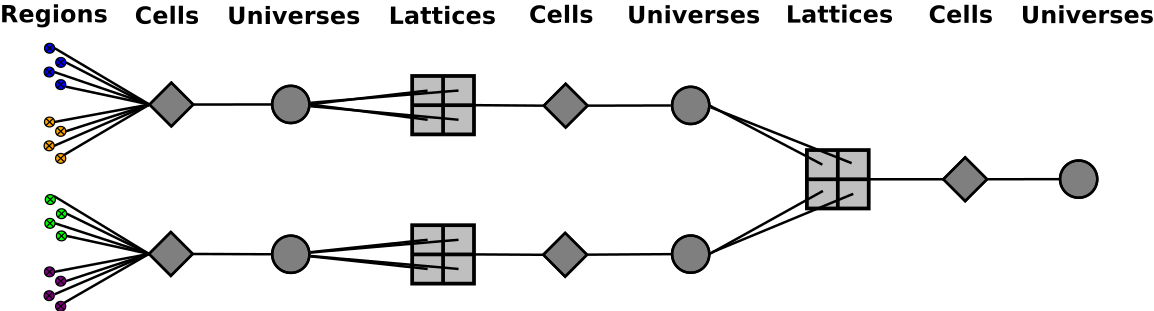
\includegraphics[width=0.82\linewidth]{figures/workflow/opencg/region-differentiation-1}
  \caption{}
  \label{fig:differentation-1}
\end{subfigure}
\begin{subfigure}{\textwidth}
  \centering
  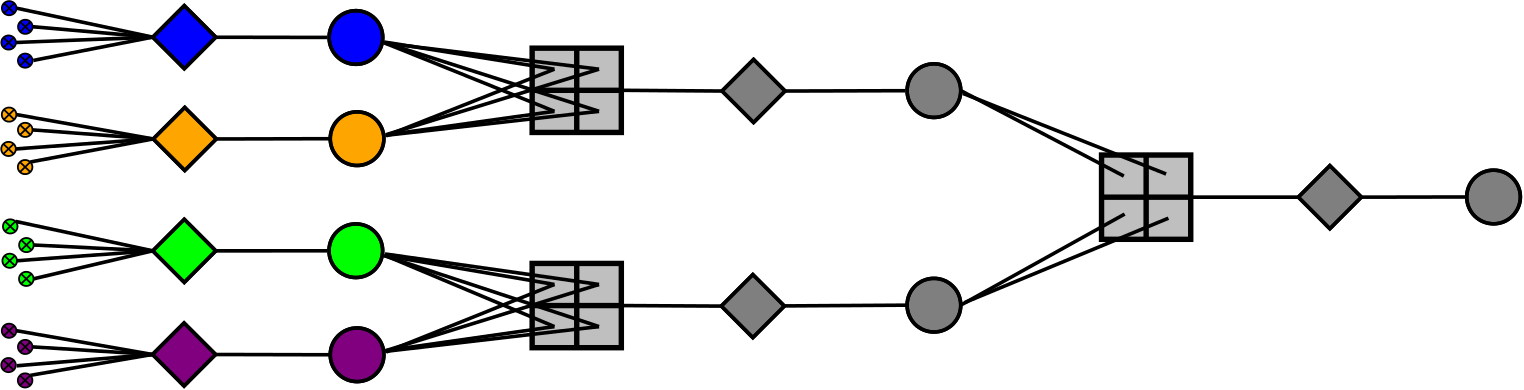
\includegraphics[width=0.75\linewidth]{figures/workflow/opencg/region-differentiation-2}
  \caption{}
  \label{fig:differentation-2}
\end{subfigure}
\begin{subfigure}{\textwidth}
  \centering
  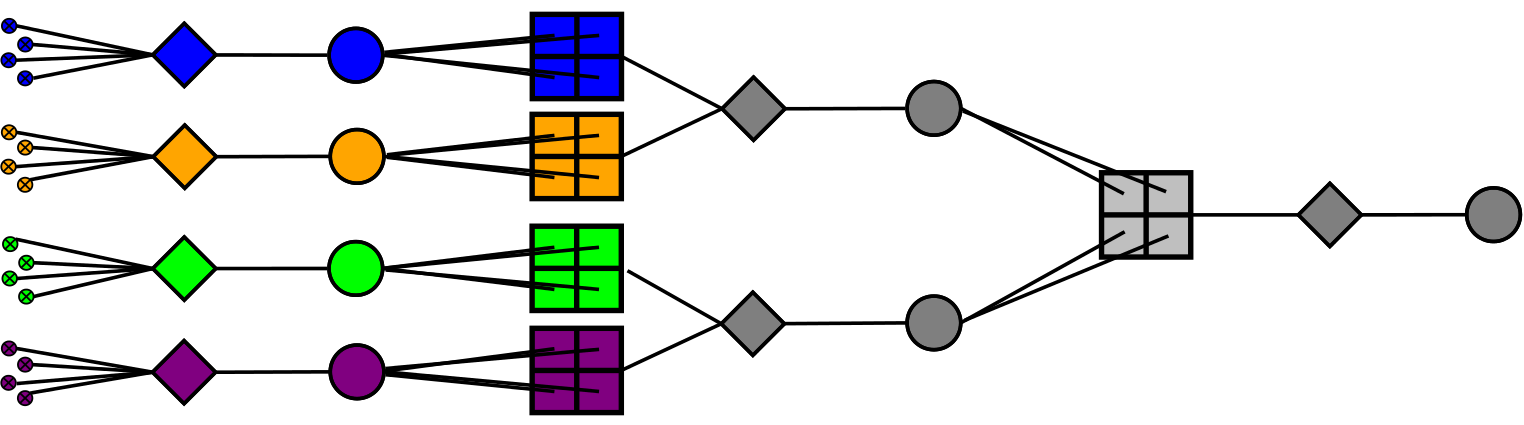
\includegraphics[width=0.75\linewidth]{figures/workflow/opencg/region-differentiation-3}
  \caption{}
  \label{fig:differentation-3}
\end{subfigure}
\begin{subfigure}{\textwidth}
  \centering
  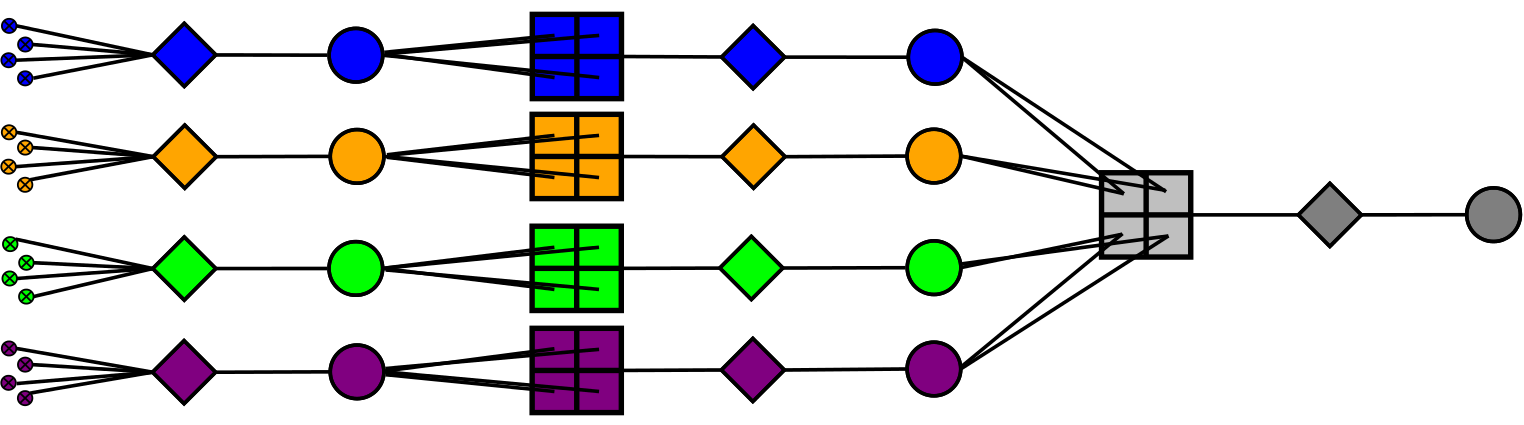
\includegraphics[width=0.75\linewidth]{figures/workflow/opencg/region-differentiation-4}
  \caption{}
  \label{fig:differentation-4}
\end{subfigure}
\begin{subfigure}{\textwidth}
  \centering
  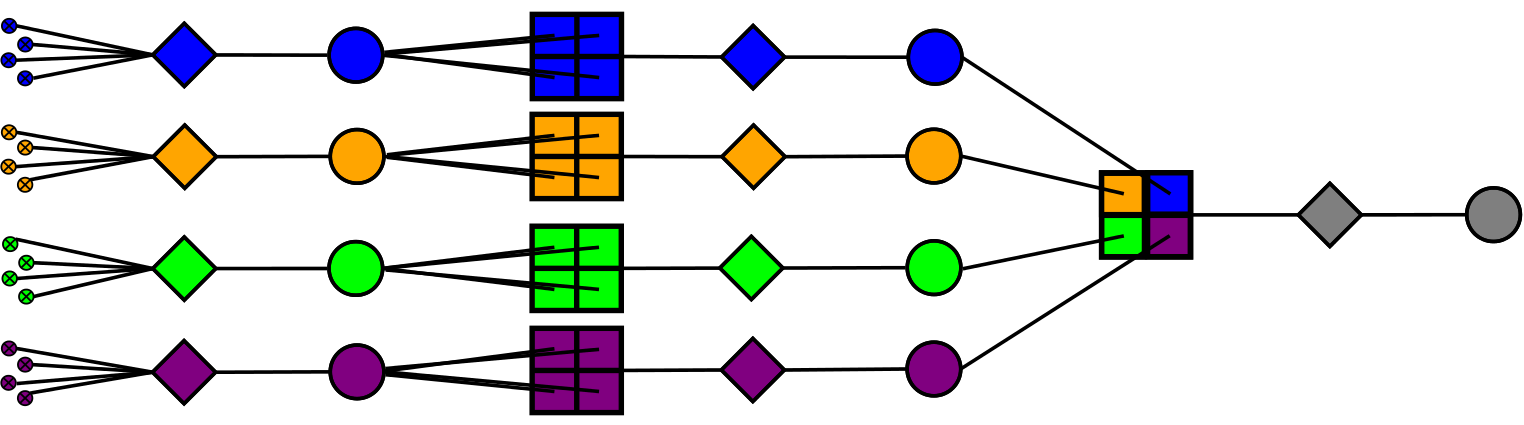
\includegraphics[width=0.75\linewidth]{figures/workflow/opencg/region-differentiation-5}
  \caption{}
  \label{fig:differentation-5}
\end{subfigure}
\caption[A few stages of the OpenCG region differentiation algorithm]{A few of the stages of the region differentiation algorithm~\cite{boyd2015opencg}. The regions (cell instances) to be differentiated are grouped and colored blue, orange, green and purple in (a). The first levels of cells and universes for each region group are differentiated in (b). The same is done for the lattices in (c). The algorithm continues to recursively differentiate cells, universes and lattices until no region groups collide at any level of the CG tree in (e).}
\label{fig:region-differentiation}
\end{figure}

The region differentiation algorithm iterates over each level of nested universes and cells. At each step, the paths for each region starting from the current level in the \ac{CG} tree and ending with the root universe node are hashed and stored in a hash table linked to the region grouping. Next, the algorithm manages \textit{primitive collisions} when two or more region groupings with the same path in the hash table point to the same primitive (cell, universe or lattice). To resolve primitive collisions, the algorithm differentiates the primitive for each region grouping involved in the collision. As primitive collisions are resolved, the algorithm merges any region groupings with paths that hash to same value in the hash table. The algorithm's termination condition is reached when the hash table only has one entry -- \textit{i.e.}, paths for all regions hash to the same value.

The region differentiation algorithm was an indispensable component of the simulation triad used to explore novel \ac{MGXS} generation techniques in this thesis. In particular, region differentiation made it possible to rapidly construct geometries to reflect the assignment of \ac{MGXS} to arbitrary collections of fuel pins for the spatial homogenization methodology introduced in Chaps.~\Crefrange{chap:benchmarks}{chap:unsupervised}. Fig.~\ref{fig:region-diff-proc-diagram} illustrates a flow diagram where the \ac{LNS} algorithm identifies the region groupings input to the region differentiation algorithm. The geometry produced from region differentiation may then be exported for use in OpenMC or OpenMOC using the compatibility modules discussed in Sec.~\ref{sec:chap4-opencg-compatibility}.

\begin{figure}[h!]
  \centering
  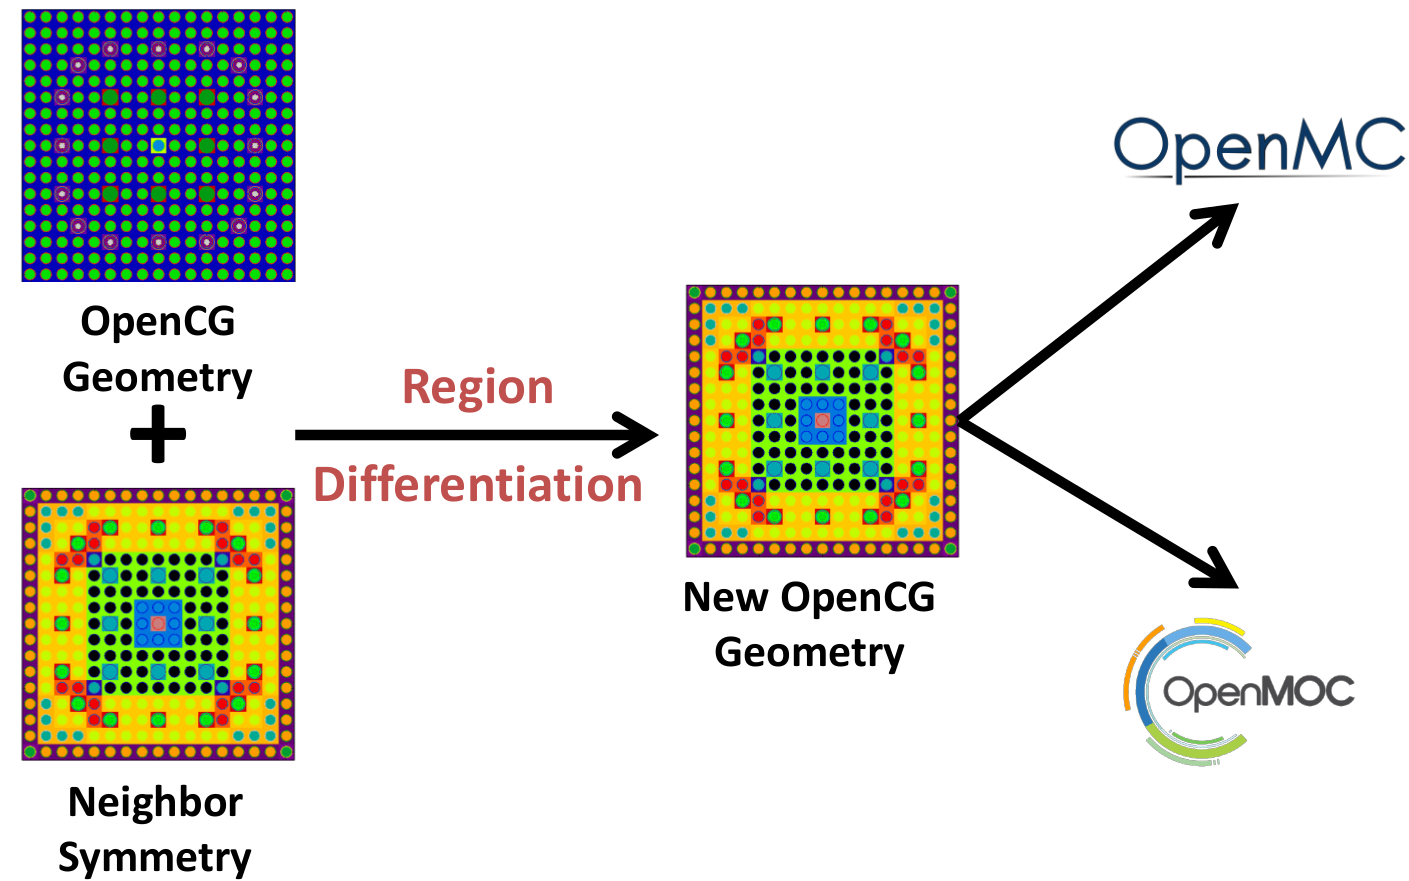
\includegraphics[width=0.8\linewidth]{figures/workflow/opencg/region-diff-proc-diagram}
  \caption[OpenCG region differentiation process diagram]{The OpenCG \ac{LNS} algorithm may be used to generate region groupings for the region differentiation algorithm to create a geometry for OpenMC or OpenMOC.}
  \label{fig:region-diff-proc-diagram}
\end{figure}
